%\documentclass[12pt,journal,draftcls,letterpaper,onecolumn]{IEEEtran}
\documentclass[conference]{IEEEtran}
\usepackage{cite}
\usepackage{amssymb}
\usepackage{amsmath}
\usepackage{graphicx}
%\usepackage[retainorgcmds]{IEEEtrantools}
%\usepackage{algorithm}
%\usepackage{algorithmic}
%\usepackage{subfigure}
%\usepackage{url}
\begin{document}
\title{Deetoo: Scalable Unstructured Search \\
	Built on a Structured Overlay}
\author{\IEEEauthorblockN{Tae Woong Choi}
\IEEEauthorblockA{Electrical and\\Computer Engineering\\
University of Florida\\
Gainsville, Florida 32611\\
Email: twchoi@ufl.edu}
\and
\IEEEauthorblockN{P. Oscar Boykin}
\IEEEauthorblockA{Electrical and\\Computer Engineering\\
University of Florida\\
Gainsville, Florida 32611\\
Email: boykin@acis.ufl.edu}
}
\maketitle

\begin{abstract}

We present Deetoo, an algorithm to perform completely general queries,
for instance high-dimensional proximity queries or regular expression
matching, on a P2P network.  
Deetoo is an efficient unstructured query system on top of existing 
structured P2P ring topologies.
Deetoo provides a reusable search tool to work alongside a DHT, thus,
it provides new capabilities while reusing existing P2P models and software.
Since our algorithm is for unstructured search, there is
no structural relationship between the queries and the network topology
and hence no need to provide a mapping of queries onto a fixed DHT structure.
Deetoo is optimal in terms of the trade-off in querying and caching cost.
For networks of size $N$,
$O(\sqrt{N})$ cost for both caching and querying is required to achieve
a constant (in $N$) search success probability.  Queries execute a time
of $O(\log^2 N)$.
\end{abstract}

%Our interest is in building efficient unstructured
%query system on top of existing structured P2P topologies.
%Deetoo provides a reusable search tool to work alongside a DHT, thus, 
%it contributes to minimize developing and deploying new P2P software.
%On the other hand, From the fact that Deetoo deals with unstructured search, 
%we can apply our network for any type of query
%without the necessity of mapping our queries onto a fixed DHT structure.
%Deetoo is optimal in terms of trade-off in querying and caching cost.
%$O(\sqrt{N}$ cost for both caching and querying is required to achieve 
%a constant search success probability. 
%Deetoo leverages $1-D$ routable small-world networks, and multicasting trees
%built on those networks, to build an unstructured query system
%which can support general queries,
%such as high-dimensional proximity queries or regular expression matching.
%We present simulation and analysis of the publishing and querying costs.
%Publishing and querying cost $O(\sqrt{N})$ bandwidth and
%run in a time of $O(\log^2 N)$ on a network of $N$ nodes.
%
%\end{abstract}

\begin{IEEEkeywords}
Peer-to-peer systems, overlay network, file searching,
query flooding, distributed systems
%multi-dimensional query, 
%scalable, unstructured, fault-tolerant, small-world network, 
\end{IEEEkeywords}
\IEEEpeerreviewmaketitle
\section{Introduction}\label{sec:introduction} 
Since the success of applications like 
Napster and Gnutella,
Peer-to-Peer (P2P) file sharing systems have become some of the most
common Internet applications. An Internet study reported
that over 73\% of all Internet traffic was 
the result of P2P file-sharing platforms\footnote{According 
to http://www.ipoque.com/}.
P2P is the single largest consumer application of bandwidth on 
networks. P2P traffic significantly outweighs Web traffic 
and still continues to grow\cite{Goth06b}.

Each node in a P2P system operates simultaneously as both a server and a client
in a distributed fashion. Nodes navigate the
underlying network without knowledge of their global structure. 
Currently, there are two common types of P2P search systems: flooding-based
unstructured systems and DHT-based key-lookup systems. 
DHT-based query systems ($O(\log N)$) outperform flooding-based systems in terms of 
search cost ($O(N)$), but they cannot support general searches.
On the other hand, flooding-based unstructured search technique can resolve 
any kind of queries at the expenxe of search cost.
The main motivation of this work is two folds: 
1) how to build optimal unstructured search system in terms of 
trade-off in caching and querying cost. 
2) how to build unstructured search system using existing structured
P2P topologies, such as Chord, to work alongside a DHT and 
to minimize developing and deploying P2P software. 

\iffalse
P2P systems may be categorized into three
different architectures: \emph{centralized},
\emph{decentralized/structured}, and
\emph{decentralized/unstructured}\cite{LCKS02}. 
First, \emph{centralized networks} rely on an indexing server for updates.
Early P2P systems such as Napster 
fall into this category. Within this architecture, each node sends
a query not to another peer, but to the central indexing server, to find
a node that matches the query. These centralized P2P
networks are clearly not scalable (unless they replicate sufficient back-up
servers) and they are not fundamentally
able to avoid the single-point of failure problem.
%A main issue in P2P applications is efficient with respect to both
%file caching and query resolution.  

\emph{Structured networks} use an overlay topology that is
structured but without central control.
In distributed hash table (DHT) based P2P overlays
\cite{is:Chord,sr:CAN,bz:Tapestry,pr:Symphony}, 
each object has a unique identification 
key that plays a role in placing an object into the network. 
A query can also pinpoint the object indexed by 
a key. DHT-based overlays are not only efficient but also partially 
resistant to failure of the nodes or links. 
The chief disadvantage of structured networks is that queries must be
mapped onto the structure of the network.  Since it is not clear (or
perhaps not possible) to map some queries onto low-dimension spaces
such as those formed by common P2P systems, not all query systems can
be easily implemented on structured networks.  An example might be
regular expression matching.  Furthermore, additional steps need
to be taken to deal with the problem of hotspots in the network, 
which form when demand for specific objects increases suddenly.

\emph{Unstructured networks} %such as Gnutella 
use flooding-based routing and random walks to locate a resource and to
resolve a query. These systems
do not require a unique key for each object.
Therefore, any type of query can be easily mapped to an
unstructured P2P system.
Unstructured systems with key-word searching are prevalent in P2P
file-sharing networks. While these systems are resilient to both node
joins and failures due to their simplicity, unstructured
file-sharing networks have a scaling problem. As the network size grows,
each participating node can become overloaded with a huge amount of
query messages, which can scale to a complexity of  $O(N)$
since all the nodes need to be visited for a single query. 
\fi
In this paper we present Deetoo, an efficient query-resolution 
algorithm based upon Kleinberg's one-dimensional construction
\cite{jk:Algorithmic}. The idea is to organize nodes in a ring in which 
each node has a set of ``local" contacts and one ``long-range" 
contact. 
A small-world model allows a reduced path discovery 
with only local information by forming a local tree in the search space. 
In addition to the search efficiency and low maintenance cost, 
we can reuse existing P2P code designed for a ring topology by adapting 
a one-dimensional small-world network model.
The heart of our work is simple data object replication and a search 
algorithm. In our model, the usual 1-D
overlay topology is transformed into a rectangular 
matrix as described in Section \ref{sec:model}.  Replication and 
query resolution are executed by bounded broadcasting over the 
columns and rows on the matrix space respectively.

This paper evaluates the novel Deetoo algorithms from a theoretical 
standpoint and through simulation. 
We focus on the behavior of the search algorithms for each of the
following metrics: successful searching probability (hit rate),
communication cost (bandwidth consumption or number of
generated messages), and search time (depth of the multicasting tree). 
Measures of the query accuracy are important because precise information 
retrieval is one of the main purposes of P2P networks. 
%Our probabilistic approach achieves $O(1)$ success rate.
Distributed systems should avoid massive communication cost. Deetoo stores 
$O(\sqrt{N})$ replicas per object with a high probability. 
Unlike the structured network, Deetoo does not require that each replicated object 
be mapped into a DHT.
A query generates $O(\sqrt{N})$ messages.
This implies more messages when compared to DHTs, which have only O($\log N$) complexity,
but offers a major improvement over flooding-based searches with
$O(N)$.

%---------------------------------------------------
\iffalse
Assume that data can be cached on $C$ of any $N$ nodes.
Since there is no structure assumed, and if load is evenly
balanced across the nodes,
caching does not depend on the data
being cached and we assume that $C$ nodes are selected at random.  Similarly,
when we query, we can check $Q$ of the $N$ nodes, again at random.  Thus the
probability we miss the stored data is approximately:
\[
\left(1-\frac{C}{N}\right)^Q = \left(1-\frac{C}{N}\right)^{\frac{N}{C}
\frac{CQ}{N}}\approx \exp(-\frac{CQ}{N})
\]
So, we need $CQ = O(N)$ in order to have a constant probability of success in
this model.  This presents an intuitive trade-off, the more nodes on which we
cache data, the fewer we need to check to find it.  To minimize $C+Q$, which
is the cost to cache an object and query for it once, the
best choice is for $C$ and $Q$ to be $O(\sqrt{N})$. 
This simple analysis
suggests that any unstructured load-balanced system will be require at least
this much communication.  Of course, logarithmic complexity would be nice, but
for many practical systems, the number of nodes might well be $100$ to
$10,000$ which mean $C$ and $Q$ values on the order of $10$ to $100$.
Such overhead costs would be completely acceptable for many applications,
 especially when we handle meta data instead of large multimedia files.
Deetoo is the first system that arbitrary unstructured queries can be mapped 
to a structured P2P system with query cost $O(\sqrt{N})$.
%--------------------------------------
\fi
Our searching algorithm can coexist on the same P2P network
with a DHT, so with Deetoo
users can still have structured as well as unstructured queries.
Also, users can control success rate and search cost with Deetoo by 
adjusting the degree of replication with a user-specified value.
In \cite{LCKS02}, Lv et al. showed that
square-root replication distribution is theoretically optimal in
terms of minimizing the overall search traffic. 
Our protocol search time outperforms other unstructured models by forming 
an efficient local tree: 
Deetoo completes searches in  
$O(\log^2{N})$ time by using Kleinberg's small-world network model.  
Lastly, due to the fact that Deetoo is built on a structured overlay,
objects can be updated or deleted after being published on the
system.  This represents an advantage over random
walk based schemes previously proposed in the literature.
%data control - deletion ability, stabilization optimal replication 
%beyond DHT - general queries
%beyond Gnutella - contrl data ( deletion, stabilization) control success rate by adjusting replication factor
%----------------------------------------------
\iffalse
The main motive of this work is three folds: 1) how to build optimal unstructured 
search systems; 2) how to build efficient generalized metric-space search systems;
3) how to build data-controllable unstructured systems which can delete replicated
object from a network or can maintain the number of replicas under frequent network 
changes (we call this \textit{stabilization}).
Currently there are two common types of P2P search systems: 
unstructured flooding based search and key based lookup provided by DHT systems.

The advantage to unstructured search is that it applies to a very wide array of 
search problems: the P2P algorithms generally put no constraint on 
the structure of the search problem itself. The downside to unstructured search is 
that due to the lack of structure, in the way the problem is posed, queries are 
necessarily more costly than structured searches such as key lookups.
Such flooding query systems are simple to implement, but
are very costly: $O(N)$ for a network of size $N$.
Another downfall of unstructured systems is that they do not have a control over 
data. Deleting replicated objects from the entire network and maintaining
number of replicas cannot easily managed by such systems.
% given by replication factor which is defined when an object is 
%inserted.

On the other hand, key lookup is highly structured and, as such, can be made to use 
logarithmic-in-network-size costs to do key lookup; however, 
many search problems cannot be mapped to the problem of key lookup.
DHT systems are much more difficult
to implement because they map the data structure of a hash table onto the structure of the P2P network. 
As such, nodes must work to maintain the global network structure to ensure that 
the data structure functions correctly.
The major advantage of the DHT is that it makes key-based lookup operations 
very cheap: $O(\log{N})$ where $N$ is the size of the network.
A major problem is mapping interesting queries onto the DHT. This is often comes down to a metric-space
embedding problem: we want to search for nearness in one metric space, but our
P2P network is defined by a second metric space. 
In many cases, no good mapping will exist. A good example is regular expression mapping. 
Regular expressions cannot, in any obvious way, be mapped to metric space.

Many common queries have no easily exploited structure. 
This work investigate an approach to use existing structure P2P systems to achieve optimal query
costs for generic queries.
%-------------------------
\fi

Deetoo provides more efficient than generic unstructured systems.  
Some of flooding-based unstructured systems with similar replication strategy or with super peers 
may achieve the same performance as Deetoo in that communication cost and query success rate. 
However, no systems can control data data objects like deleting or stabilizing objects easily in our best knowledge.
Deetoo also has ability to maintain replication rate by stabilization even if network size changes.
which can not be easily done by most of current unstructured systems.
By the nature of unstructured systems, Deetoo can map any kind of search problem to its structure.


The rest of this paper is organized as follows: First, our searching
algorithm is compared with that of the recent routing schemes in the following section. 
In Section \ref{sec:model}, the system model
used in this work is described. We analyze the performance of Deetoo in
Section \ref{sec:analysis}. In Section \ref{sec:simulation}, we present
simulation results of the performance of Deetoo. Finally, conclusions are 
drawn in Section \ref{sec:conclusion}.

\section{Related Works}
\label{sec:related_works}
Highly structured P2P networks with DHT look-up algorithms 
\cite{is:Chord, sr:CAN, bz:Tapestry, pr:Symphony} 
are efficient in that these networks achieve low query costs. This is 
because they place data objects at particular points on the network topology
which are determined by an object's key. Beehive\cite{re:beehive04} 
achieves constant look-up latency on top of a
DHT through proactive replication. Despite their efficiency, the possibility 
of operation, even with extremely unreliable nodes, has not been yet
examined. In addition, it is impossible for Beehive to handle
high-dimensional complex queries.  Extensive research has been conducted 
to address the limits of the exact search problems in DHT.
%more works need to be included (interest-based clustering, distributed kd-tree)
%ex. semantic clustering (SSW)
One example is \emph{pSearch}.\cite{psearch}
In \emph{pSearch}, semantic indices are mapped to a CAN overlay. 
A \emph{rolling index} reduces the number of dimensions for mapping purposes 
onto the overlay and divides the semantic vector(SV) into sub-vectors. 
Each sub-vector has the same number of dimensions as a CAN overlay does.
Although \emph{pSearch} is simple and supports high-dimensional queries, 
the \emph{rolling index} generates additional cost to publish the index and search 
because the operations for publishing and searching are repeated \textit{p} times.
\emph{Cubit}\cite{cubit} provides keyword search capability over a DHT. \emph{Cubit} 
efficiently finds multiple closest data sets for a given query. However, 
it requires the creation of a keyword metric space and only returns multiple similar results
to compensate for typos in queries. Deetoo does not demand any keyword mapping 
into DHT and can execute more general queries like regular expression searches.

%flooding
Unlike DHTs, unstructured P2P systems mostly depend on flooding 
for message transfers. The big advantage of flooding-based P2P systems 
is the capability of high-dimensional search.
The early version of Gnutella was based on naive
flooding. Because flooding produces a very large number of
messages over an entire 
network, pure flooding limits network size. 
To address this scaling problem, various types of solutions have been 
proposed. KaZaa\cite{kazaa} and iXChange
\cite{JohnstoneSM05} introduced central server-like super-peers. 
However, super-peers cause bottle-necks, security issues, and the single 
point of failure problems due to their server-like characteristics. 
Recently, research efforts have also focused on locality-based flooding. Systems 
adopting interest-based locality\cite{Guo04,Guo05,SMZ03} assume that 
two peers having common interests share pieces of a data object. 
Under this assumption, a shortcut 
connection is established between two peers having common interests, 
and queries from one peer are delivered to the other through this 
shortcut link in the first stage of flooding. 
Locality-based flooding requires warm-up procedures to gather query 
history for shortcut connections. 
\textit{LightFlood}\cite{JiangGZW08} uses 
a neighbor-degree-based locality scheme. 
\textit{LightFlood} forms a tree-like sub-overlay called 
\textit{FloodNet} using neighbors' degree information. Once the sub-overlay 
is formed, there are two overlay networks in the system: the original 
P2P overlay and \textit{FloodNet}. The flooding takes two stages.
Messages are transmitted using pure flooding with relatively small TTL values 
in the first stage. The peers that receive the query with zero TTL trigger 
the second stage of flooding in the \textit{FloodNet}. Although 
\textit{LightFlood} is simple and helps stop generating massive messages 
for queries at a certain point, searching unpopular objects requires  
the entire network to be visited; in addition, \textit{LightFlood} needs to 
be warmed up.  

A random walk based search technique is introduced by Adamic et. al. 
in \cite{alph:powerlaw01}. 
Their work reduces search cost by the factor of the number of replicas, 
but they do not consider replica placement. 
Although random walk search has an advantage over flooding
in terms of search cost, it has some
scalability problems because almost all the queries tend to concentrate
on the high degree nodes. To address this problem, object
replication with square-root principle\cite{CohenS02,LCKS02}
and topology reconstruction\cite{Cooper05} have been proposed. 
Both reduce search time but incur considerable communication cost 
to maintain fresh topologies or data replication copies. 
Popularity-biased random walk\cite{zs:popularity06}
achieves square-root principle without the cost of data movement or
topology reconstruction. Sarshar et al. \cite{ns:percolation}
combined flooding and random walking in power-law networks. In their
work, a query can be resolved in time $O(\log N)$. However
$O(N\times \frac{2log k_{max}}{k_{max}})$ messages are
transmitted for a single query, where $k_{max}$ denotes the maximum
degree; thus, when $k_{max} = \sqrt{N}$ this becomes $O(\sqrt N \log N)$.

Liu et al. \cite{LiuHZ04} study bounded broadcasting in wireless sensor networks. 
A balanced push and pull strategy achieves $O(\sqrt N)$ search 
cost in the best scenario. However, the \emph{comb-needle data discovery} technique 
requires nodes to estimate cache and query frequency.
All nodes in the network should keep their location information in the grid. 
Though they do not analyze search time, it is possible to estimate it. By the
nature of the hop-by-hop message transfer, the \emph{comb-needle data discovery} 
takes linear time in the bounded range which is $O(\sqrt N)$. 
The \emph{dynamic paths} quorum system\cite{Naor05} 
is scalable and operates in a dynamic setting. The quorum sets are 
divided into reading quorums and writing quorums in a grid, and each 
reading quorum intersects each writing quorum. Naor et al. analyzed probe 
complexity and availability, especially in a dynamic environment. 
The probe complexities of the non-adaptive (without stabilization)
and adaptive (with stabilization) algorithms is 
$\Theta(\sqrt N \log N)$ and $\Theta(\sqrt N)$, respectively. 

\section{The Deetoo Search Algorithm}\label{sec:model}
In this section we describe the data structure and search algorithm
we use for Deetoo.  We take a similar approach to the idea of DHT P2P networks: take the hash table
data structure, and build a distributed data version of this data structure
where memory locations spread across many nodes.  
To understand the Deetoo P2P system, we will first describe a local
data structure and then describe a distributed version of that data structure.

\subsection{An unstructured ``hash" table}
\label{sec:localtab}

Consider a table data structure that has $B$ bins arranged in a $k\times l$
array ($B=kl$).  We can say $b_{ij}$ is the bin in row $i$ column $j$.  To add an
object into this table, select a random column and insert the object into each
bin in that column.  Which is to say, choose a random value $r\in (1,l)$,
and insert the object in the set of bins $C_r = \{b_{ir} | i \in (1,k)\}$.
To search for an object, select a random row and check each bin in that
row for the
object.  Equivalently, choose a random value $p \in (1,k)$ and look
for the object in the set of bins $Q_p = \{b_{pj} | j \in (1,l)\}$.  Since
every row and column intersect at exactly one bin, $C_r \cap Q_p = \{b_{pr}\}$,
a query will always find
one bin into which an object was inserted.  The number of bin accesses to
insert an object is $k$.  The number of bin accesses to query for an object is
$l$.  A trade-off between cost of insertion and cost of searching exists.

As a local data structure, the above may have little value: it costs $k$ times
more to store than an unsorted list, and the total number of comparisons
needed for a search is still $M$ if there are $M$ objects in the table.
However, as a distributed data structure designed to distribute load and
minimize communication, it is useful since only $l$ bins need to be searched.
This data structure achieves totally balanced load distribution 
in the network because each object is replicated over a bounded region 
irrespective of its popularity. On current unstructured systems, queries 
can concentrated on a specific peer having many objects. Besides, popular objects 
are likely to be available at several nodes and the probability of succeeding in
queries for it is much higher. In other words, queries for rare
objects are barely 
answered. Because our algorithm distributes objects 
evenly over the network, we can avoid creating \emph{hotspots} and improve 
probability of finding rare objects.
In the next section we describe how to
make a distributed version of this data structure which can support general
data objects and queries.  We will describe a randomized version of the above
where queries succeed with a high probability.
\begin{figure}
\centering
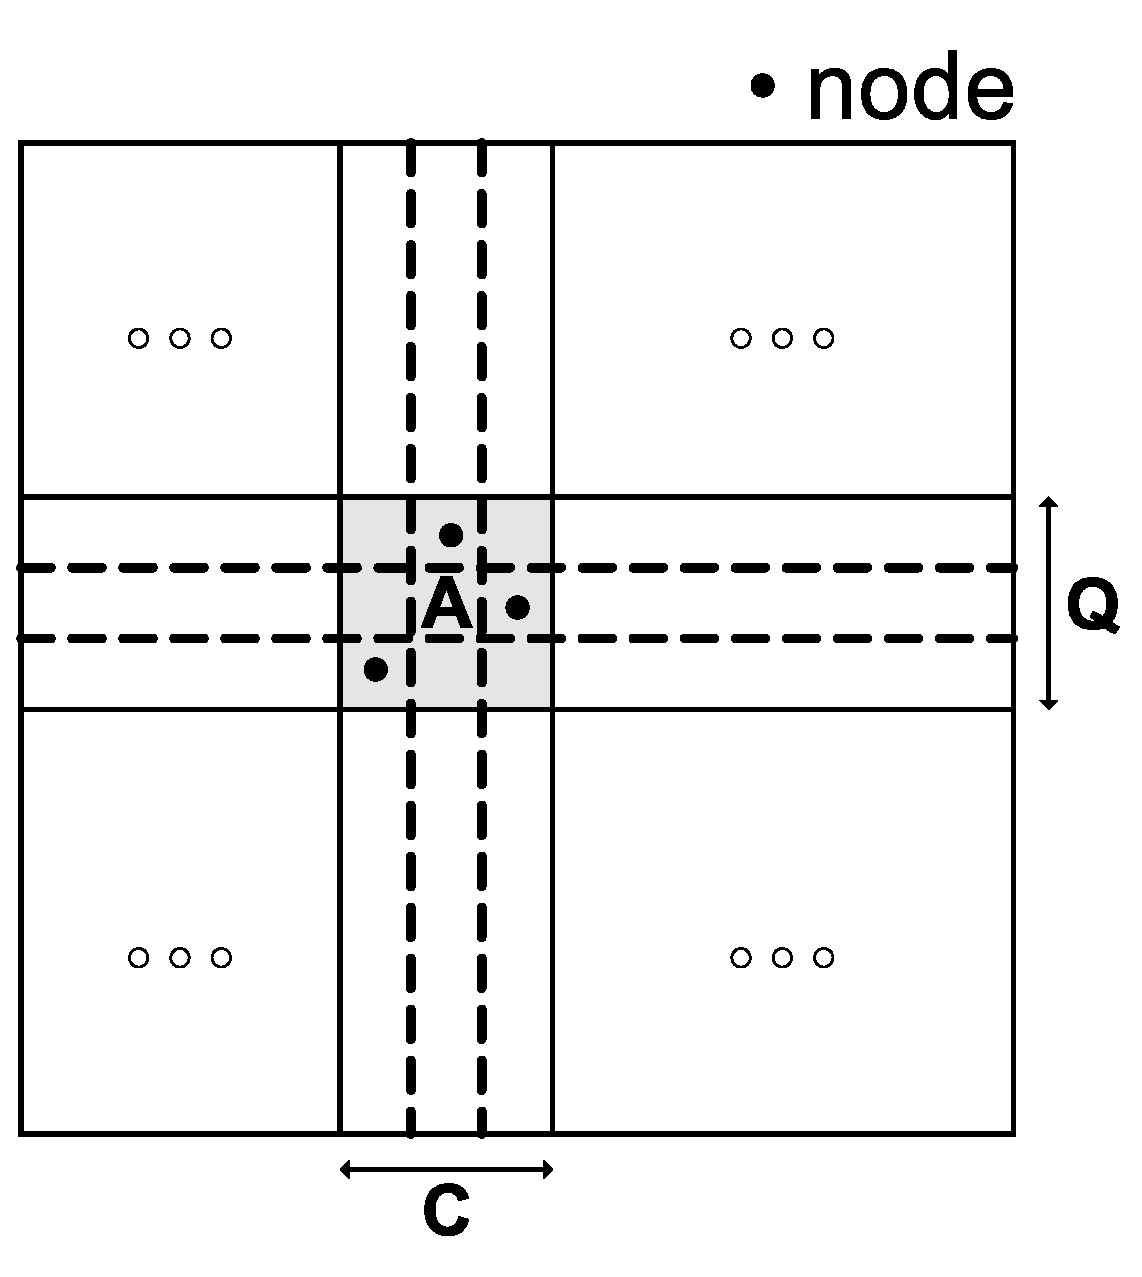
\includegraphics[width=2.5in]{space}
\caption{The caching and querying space.} \label{fig:space}
\end{figure}

\subsection{A Distributed unstructured table}
\label{sec:table}
Our setting will be the standard P2P setting: there are $N$ nodes which can
communicate, store objects and perform queries.  In addition to nodes, there
are also bins.  Bins may or may not be occupied by a particular node.  The
number of bins is assumed to be fixed at some very large number, for instance
$2^{160}$.  The bins are arranged in a rectangular array, which in this work
we will assume to be square.  In the data structure of
Section \ref{sec:localtab}, each row and column intersect at exactly one
bin that may or may not be occupied by a node.  Instead of
querying and inserting along one row and one column, we will do so over a
sufficient number of rows and columns such that the probability of having 
more than one node in the overlapping set is very likely to be one.
\begin{center}
\begin{figure*}[ht]
\centering
\begin{tabular}{c|c|c}
\begin{minipage}[t]{2.1in}
\centering
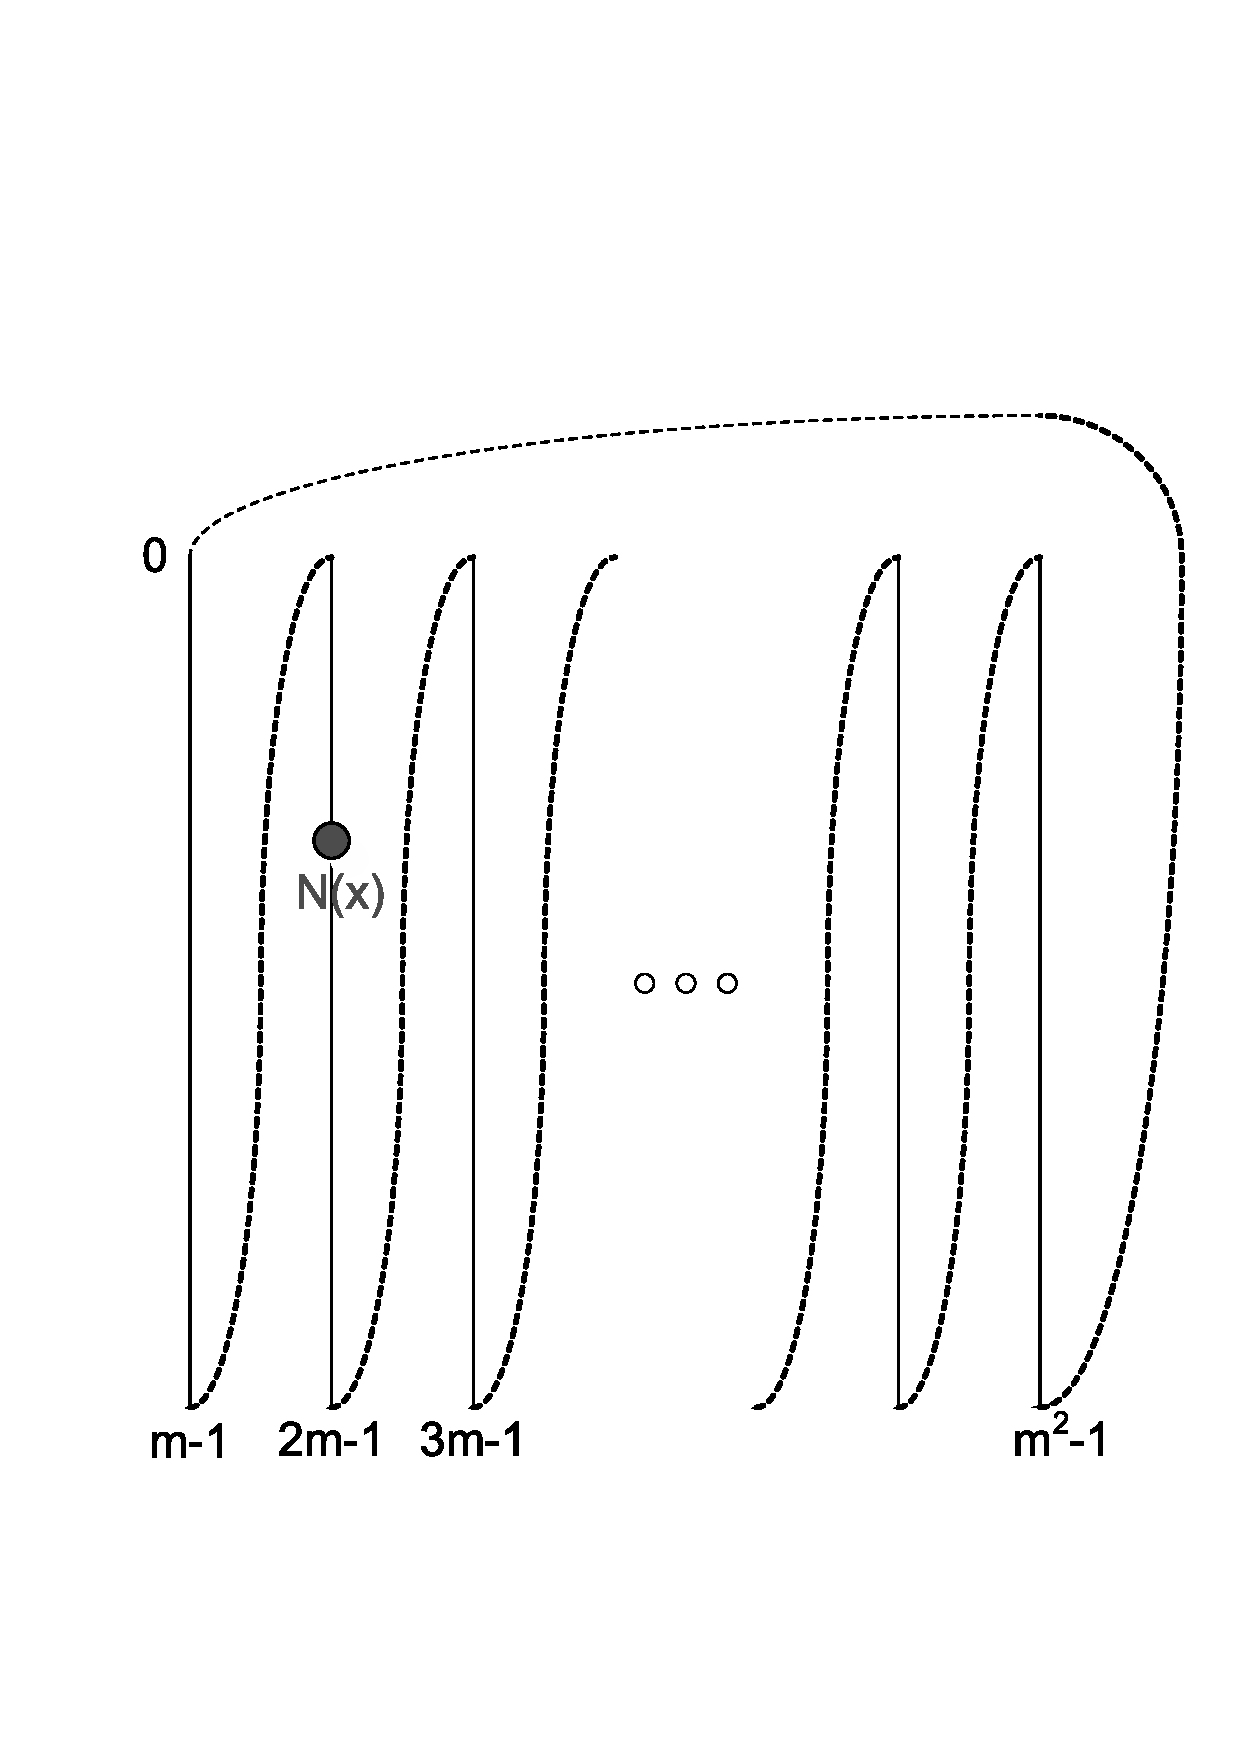
\includegraphics[width=1.5in]{cache}
\caption{Virtual ring 1 for caching.}
\label{fig:cache}
\end{minipage}
& \begin{minipage}[t]{2.1in}
\centering
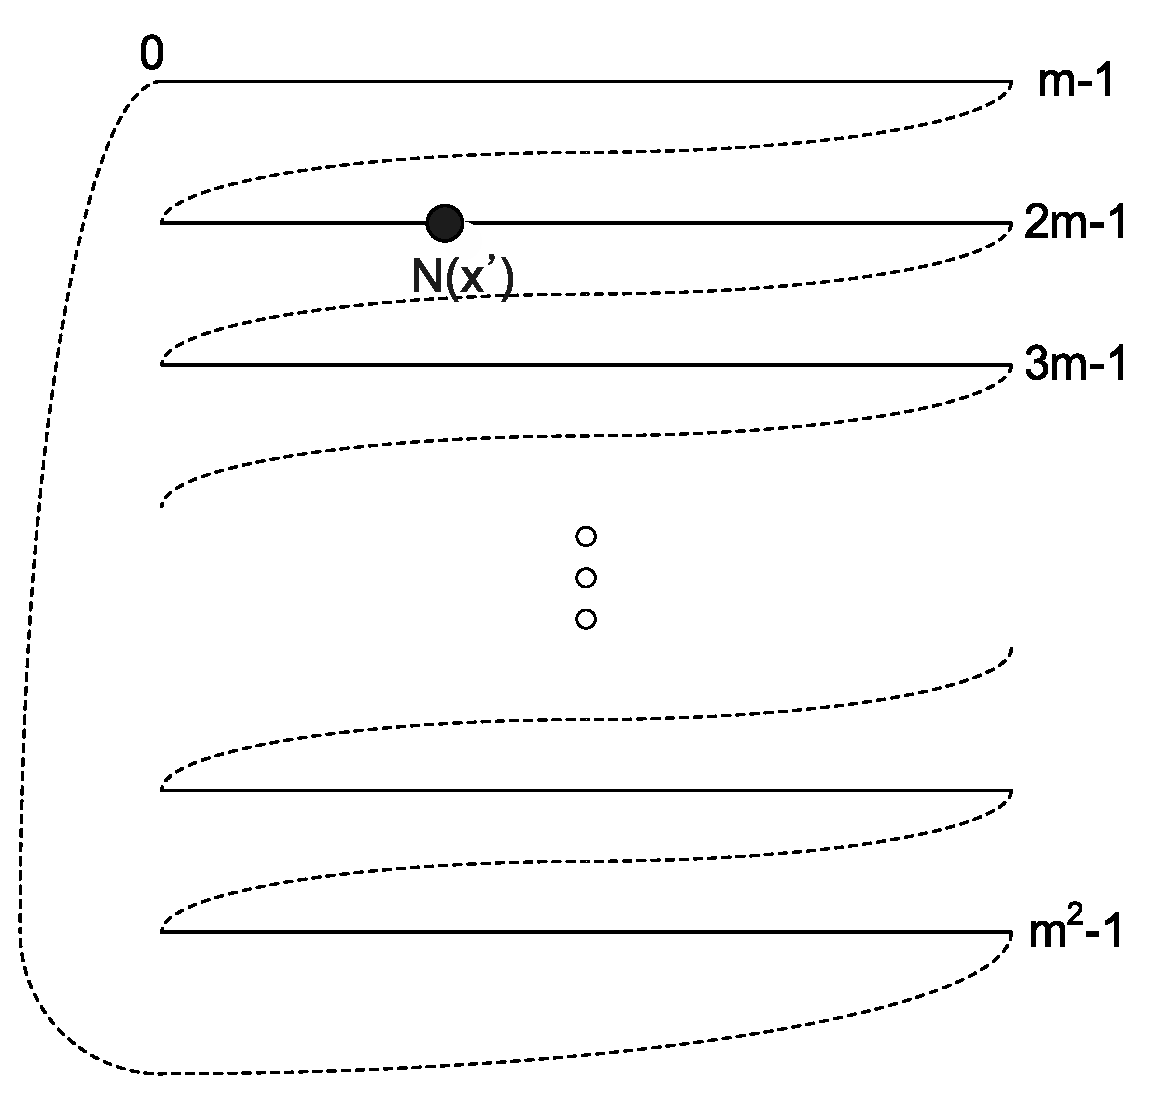
\includegraphics[width=1.5in]{query}
\caption{Virtual ring 2 for querying.} \label{fig:query}
\end{minipage}
& \begin{minipage}[t]{2.1in}
\centering
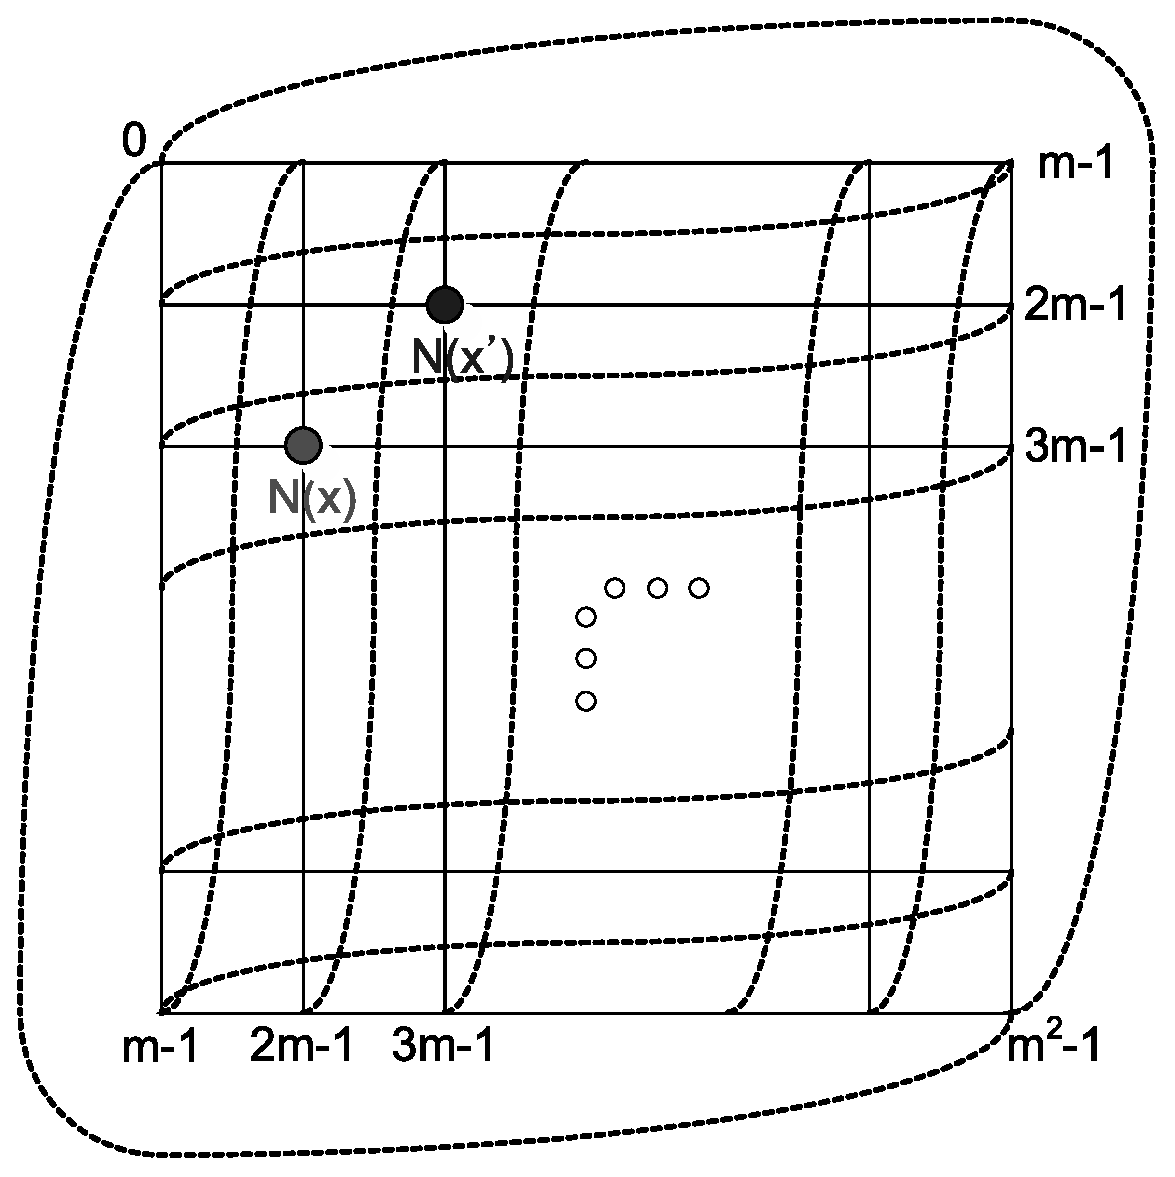
\includegraphics[width=1.5in]{combined}
\caption{The complete searching space.} \label{fig:combined}
\end{minipage}\\
\end{tabular}
\end{figure*}
\end{center}
Figure \ref{fig:space} depicts the $2-D$ array we use to cache (insert)
and query (search).  In Figure \ref{fig:space}, the area \textit{A} represents the
intersection of a particular cache and query operation.  We see in that
area, for example, there are three nodes, and so the query will be successful.  We need to
show several things to see that this algorithm will work in a distributed
setting:
\begin{enumerate}
\item Show how to efficiently send cache and query messages to entire columns
and rows respectively.
\item Show how to deal with nodes joining and leaving the network.
\end{enumerate}

To deal with the above two problems we leverage existing work on building
routable $1-D$ P2P networks such as Chord\cite{is:Chord} and the small-world
model\cite{jk:Algorithmic}.  Rather than build a P2P network that is
explicitly two dimensional, we build two sub-graphs, each of which is a 1-D 
ring, which we can call the query ring and the cache ring.  Each P2P 
node has exactly one address, and hence position, on each ring.  This is
depicted in Figures \ref{fig:cache}, \ref{fig:query}, and \ref{fig:combined}; 
these drawings illustrate how one-dimensional rings for querying and caching 
locally overlay atop of the 2-D Deetoo array.
A node is cached at location $i$ with probability $c_{i}$ and a
query node is placed at location $i$ with probability $q_{i}$ in the query ring. 
$N(x)$ and $N(x^\prime)$ denote nodes whose addresses are $x$ and $x^\prime$, respectively.
$x^\prime$ is transposed address of $x$.

In order to achieve the effect of ordering the cache ring by increasing
along the columns and the query ring to increase along the rows, the bin
address for a given node in the query ring must be the transpose of the
address on the cache ring, as depicted in Figures \ref{fig:cache} and \ref{fig:query}.  
Assume that the size of the address space,
and hence number of bins, is $B=m^2$.
The address mapping algorithm is as
follows: Let $x$ denote an address on the cache ring. The address
$x$ can be expressed by
column element, $x_{i}$, and row element, $x_{j}$, such
that $x = m x_i + x_j$.
A translated address on the query ring $x^\prime$ is obtained by exchanging
column element and row element:
$x^\prime = m x_{j} +x_{i}$.

So, each P2P node then has two addresses in virtual 1-D rings and follows the usual
procedure for joining each of the two rings as described in \ref{sec:join}.
Notice that on the cache ring, the nodes in the same columns (and adjacent
columns) have adjacent addresses.  On the query ring, nodes in the same row
(and adjacent rows) have adjacent addresses.  Because the rings are efficiently
routable, it is also efficient to send a message to a randomly selected node near
the start of a column or row.  Similarly, to reach all elements of a row or
column, we can use a bounded broadcast on one of the two rings.  

\subsection{Bounded Broadcast}
\label{sec:broadcast}

In Deetoo, a bounded broadcast is accomplished with the following 
recursive algorithm:  
To broadcast a message over the region $[x, y]$, 
our routing algorithm finds any node in the given range firstly via greedy routing,
in which a node finds the closest node to the destination as its next node.
Let us assume that a node $x$ is the first node in the range recognized by greedy routing, 
then the message is sent to node $x$. 
Suppose $x$ has $F$ connections to nodes in the range $[x, y]$. 
We denote the $i^{th}$ such neighbor as $b_i$.
The node $x$ sends a bounded broadcast over a sub-range, 
$[b_i, b_{i+1})$, to $b_i$, except the final neighbor. 
Differently stated, $b_i$ is in charge of bounded-broadcasting 
in the sub-range $[b_i, b_{i+1})$. If there is no connection to a node in the sub-range, 
the recursion is ended and the node stays in the tree as a leaf node.
To the final
neighbor ($b_F$), $x$, sends a bounded broadcast to $[b_F, y]$.
When a node receives a message to a range that contains its own address
the message is delivered to that node in addition to being routed to others.
Figure \ref{fig:tree} shows how this bounded broadcast forms a local 
tree recursively. The time required for this is $O(\log^2 N)$ as 
shown in Section \ref{sec:search_time}.
By Deetoo's recursive bounded broadcasting algorithm, all nodes in the range 
are involved in forming the local tree because only a node with no connection 
in the sub-range to the node which is responsible for bounded-broadcasting 
can stop recursion out of each branch of the tree.

\begin{figure}
\centering
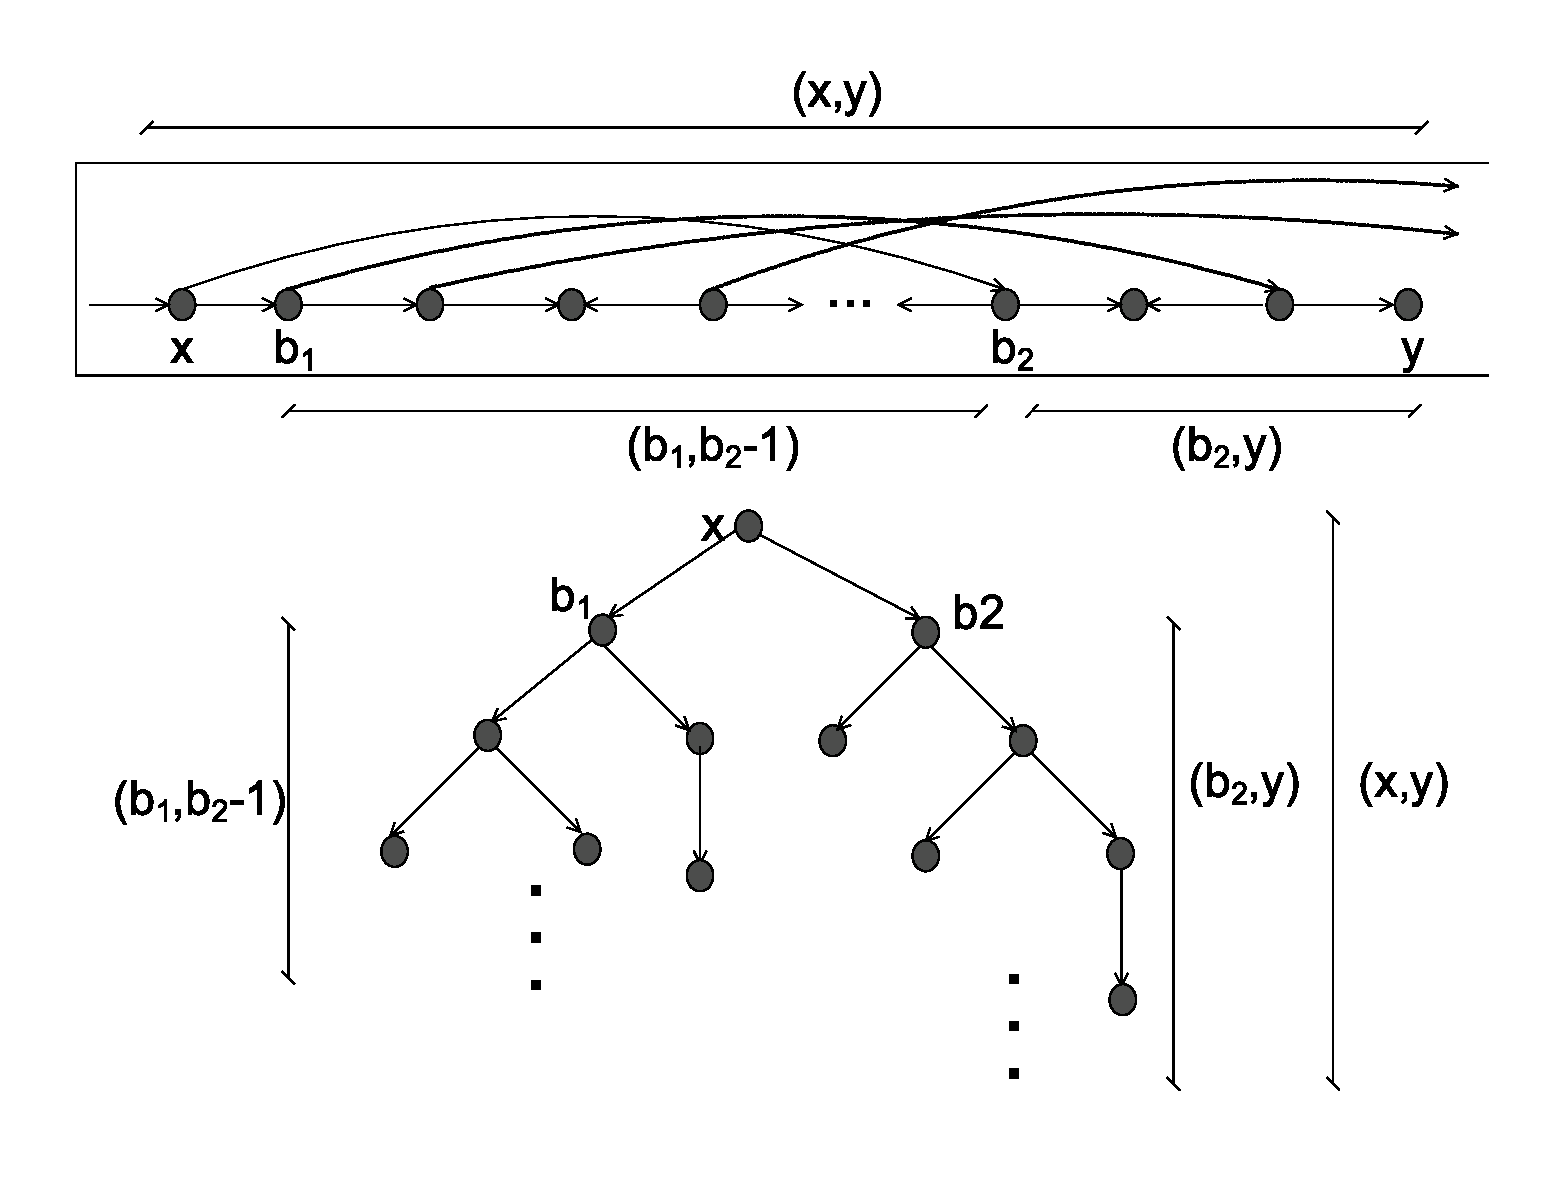
\includegraphics[width=3.0in]{tree}
\caption{Bounded Broadcast in range $[x, y]$} \label{fig:tree}
\end{figure}

\subsection{Data Insertion and Query}\label{sec:cache}
Deetoo is a search algorithm on a specific network structure. When an object
is inserted at a node $a$ as in Figure \ref{fig:cache1}, 
Deetoo selects, at random, a range in which a query message is to be broadcasted 
locally. Node $a$ starts greedy routing to find a node 
$n$ in this random range and $n$ starts bounded broadcasting 
within a limited range on the caching ring to replicate the object
(Figure \ref{fig:cache2}). 
Bounded broadcasting size for caching ($C$) is given by
$C=\alpha \sqrt{\frac{B}{N}}$, where $\alpha$, a replication factor, is a
constant(details about this formulation is followed in Section
\ref{sec:analysis}). All nodes in the range of bounded broadcasting 
eventually receive a copy of an object, $o$ (Figure \ref{fig:cache3}).

Query resolution follows the same bounded broadcasting steps. The only
difference is that the query resolution is executed in the querying
space in which every node's address is transposed (stated  
in Section \ref{sec:table}) in
the caching space. Bounded broadcasting size for a query, $Q$,
follows the same formulation as the caching size $C$ as shown above. Figures
\ref{fig:query1}, \ref{fig:query2}, and \ref{fig:query3} show the
steps involved in a query: node $a^\prime$ issues a query, node $n^\prime$ initiates a 
bounded broadcast, and node $n(o)$ resolves a query. Since all nodes in the area
\textit{A} have a copy of an object $o$, $n^\prime$ can retrieve
a desired object from any of the nodes in \textit{A}. By following these
steps, a query can be resolved if at least one node exists in
\textit{A}. Note that a user can select bounded broadcasting size by adjusting 
the \textit{replication factor}, $\alpha$. The bigger the $\alpha$, 
the higher the probability to hit a node in \textit{A}, at the expense of 
larger number of messages and replicas. 

\begin{center}
\begin{figure*}[ht] 
\centering
\begin{tabular}{c|c|c}
\begin{minipage}[t]{2.1in}
\centering
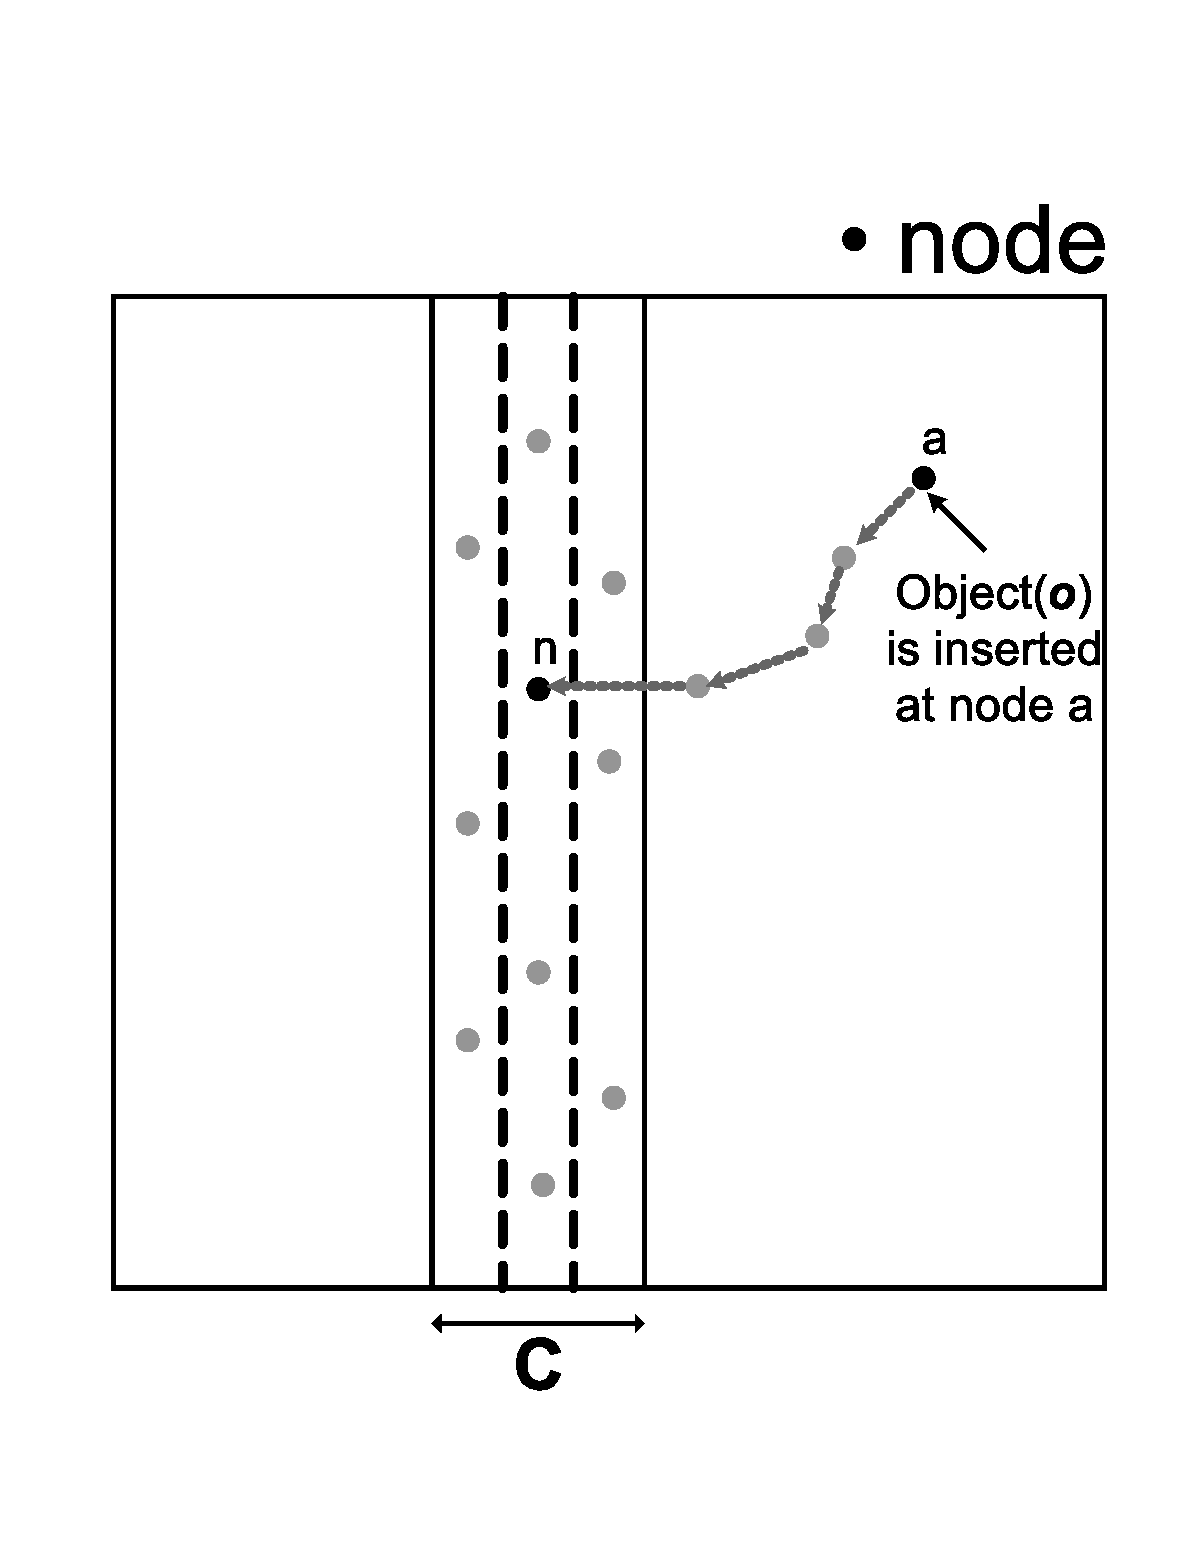
\includegraphics[width=1.4in]{cache_1}
\caption{An object(\textit{o}) is inserted at node \textit{a}. 
The message is routed to a node(\textit{n}) in the 
region for the bounded broadcast.}
\label{fig:cache1}
\end{minipage}
& \begin{minipage}[t]{2.1in}
\centering
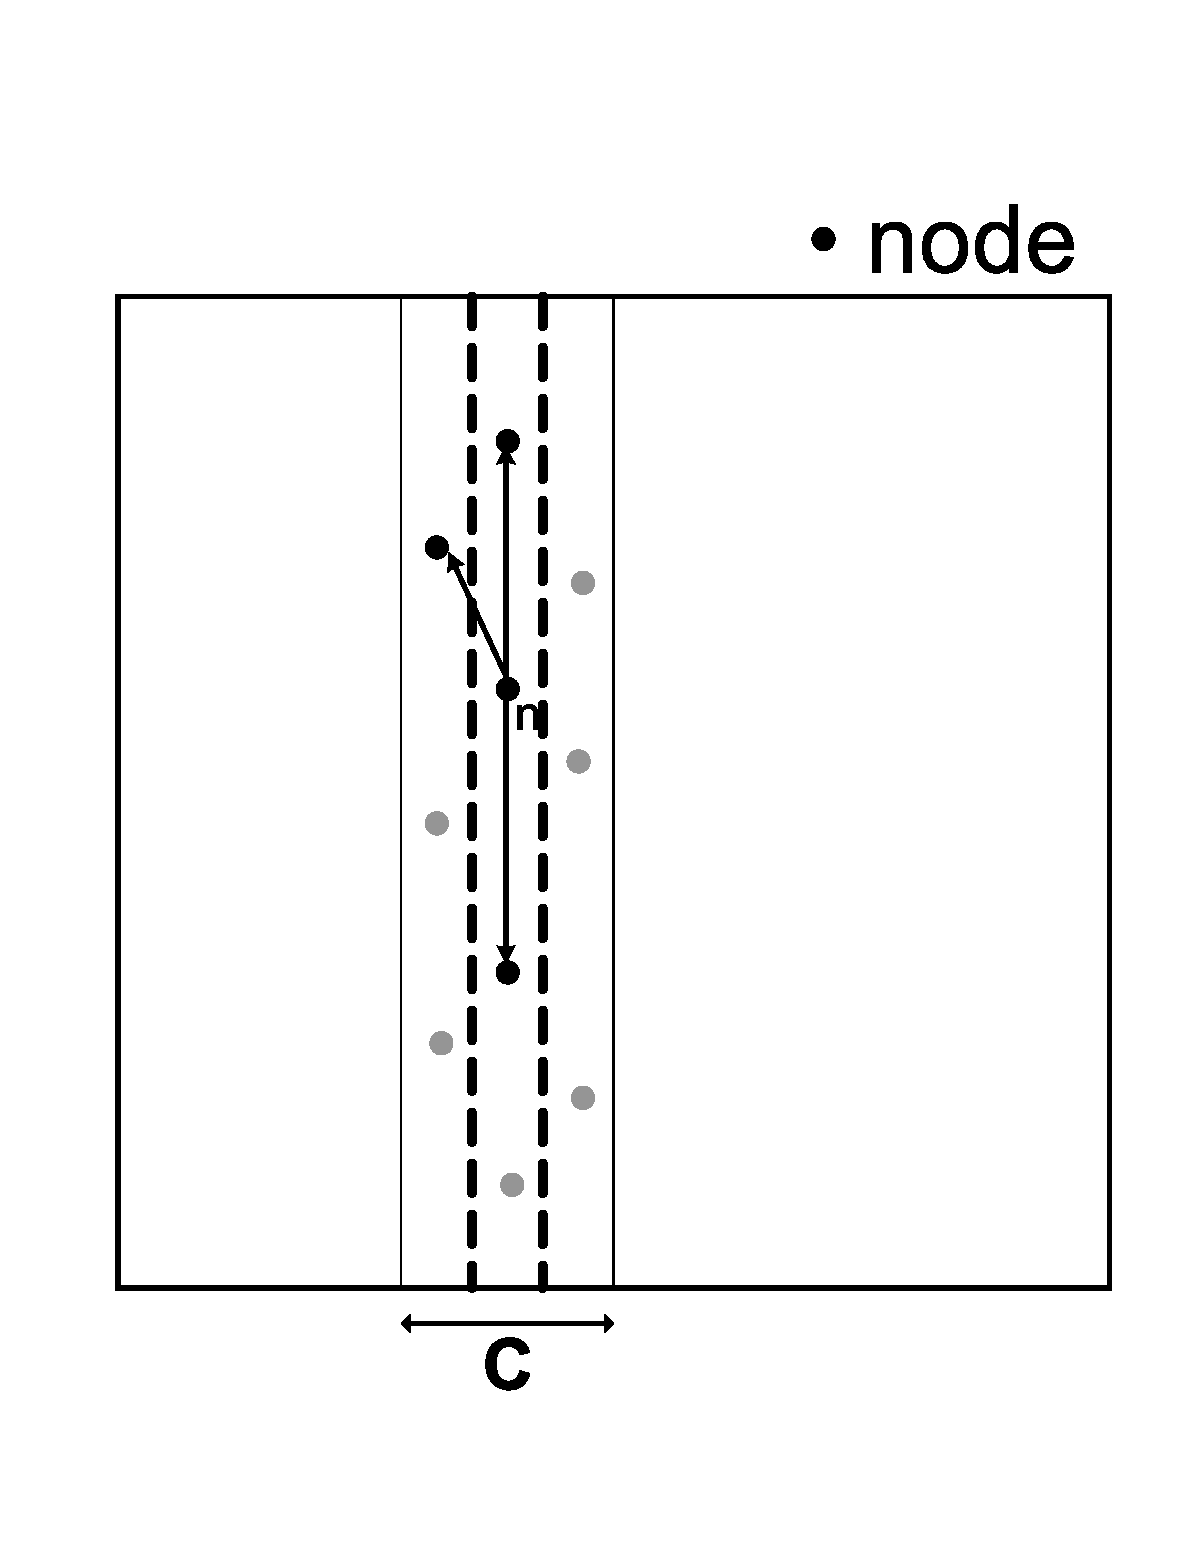
\includegraphics[width=1.4in]{cache_2}
\caption{The bounded broadcast starts at node \textit{n}.}
\label{fig:cache2}
\end{minipage}
& \begin{minipage}[t]{2.1in}
\centering
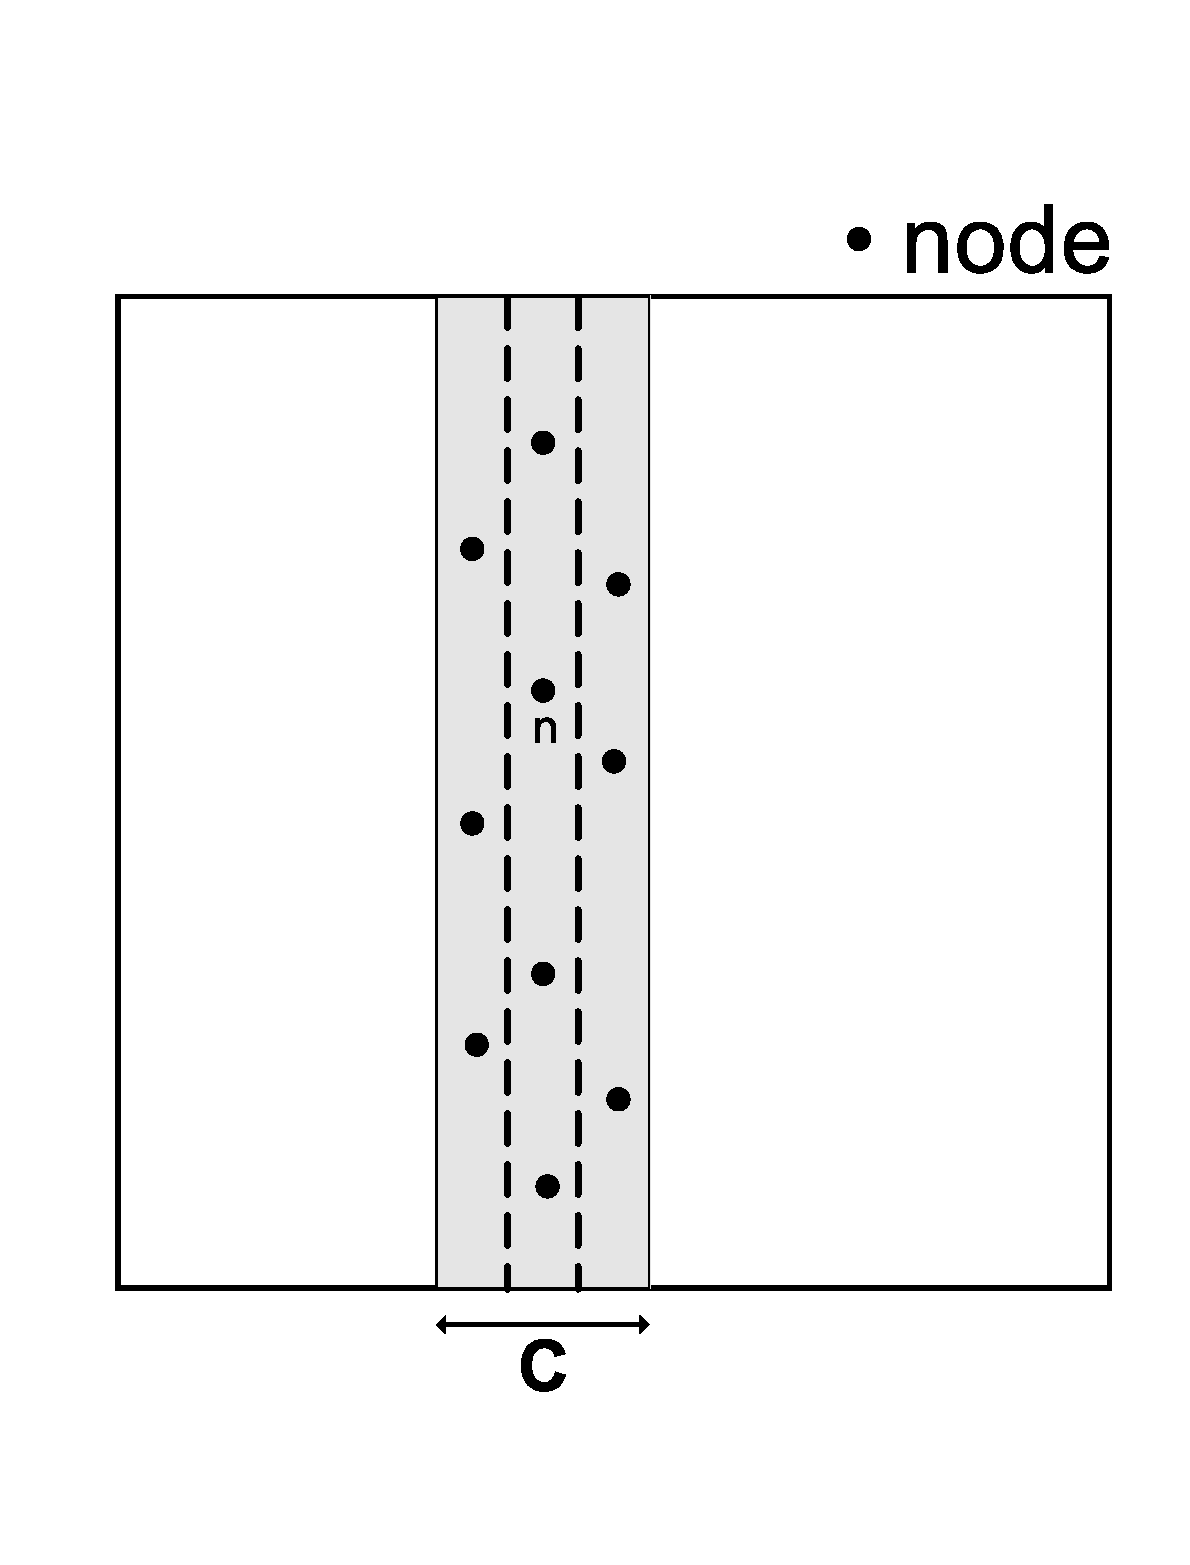
\includegraphics[width=1.4in]{cache_3}
\caption{All nodes in the range receive the message.} \label{fig:cache3}
\end{minipage}\\
\end{tabular}
\end{figure*}
\end{center}

Users may want to insert objects into a network, or delete them from a network.
The following explains how Deetoo manages both insertion and deletion.
\begin{itemize}
\item \textbf{Object Insertion: } When a new object is inserted to the network,
copies of the object are created along some sets of columns in the matrix
space (the number of columns is inversely proportional to the square-root
of the network size) using bounded broadcasting. Unlike a DHT, each object does not have to have a
unique identification number, and each inserted object does not have
to map a key to the ``closest" node.

\item \textbf{Object Deletion: }Objects do not stay forever in the networks.
When an object is obsolete, Deetoo provides a deletion that uses both 
caching and querying.
First, a query for an object which needs to be deleted is performed in order 
to retrieve the object's range. Note that each object writes its range information 
in itself or its meta data when it is cached. After the object's range is acquired, 
the \emph{deletion} message is broadcasted within the range in the same way the object
was cached. As a result, Deetoo guarantees all replicated objects that are 
supposed to be stored in the nodes in the range to be removed.
%\item Join cost (show effetiveness of data insertion and deletion)
\end{itemize}

\begin{center}
\begin{figure*}
\centering
\begin{tabular}{c|c|c}
\begin{minipage}[t]{2.1in}
\centering
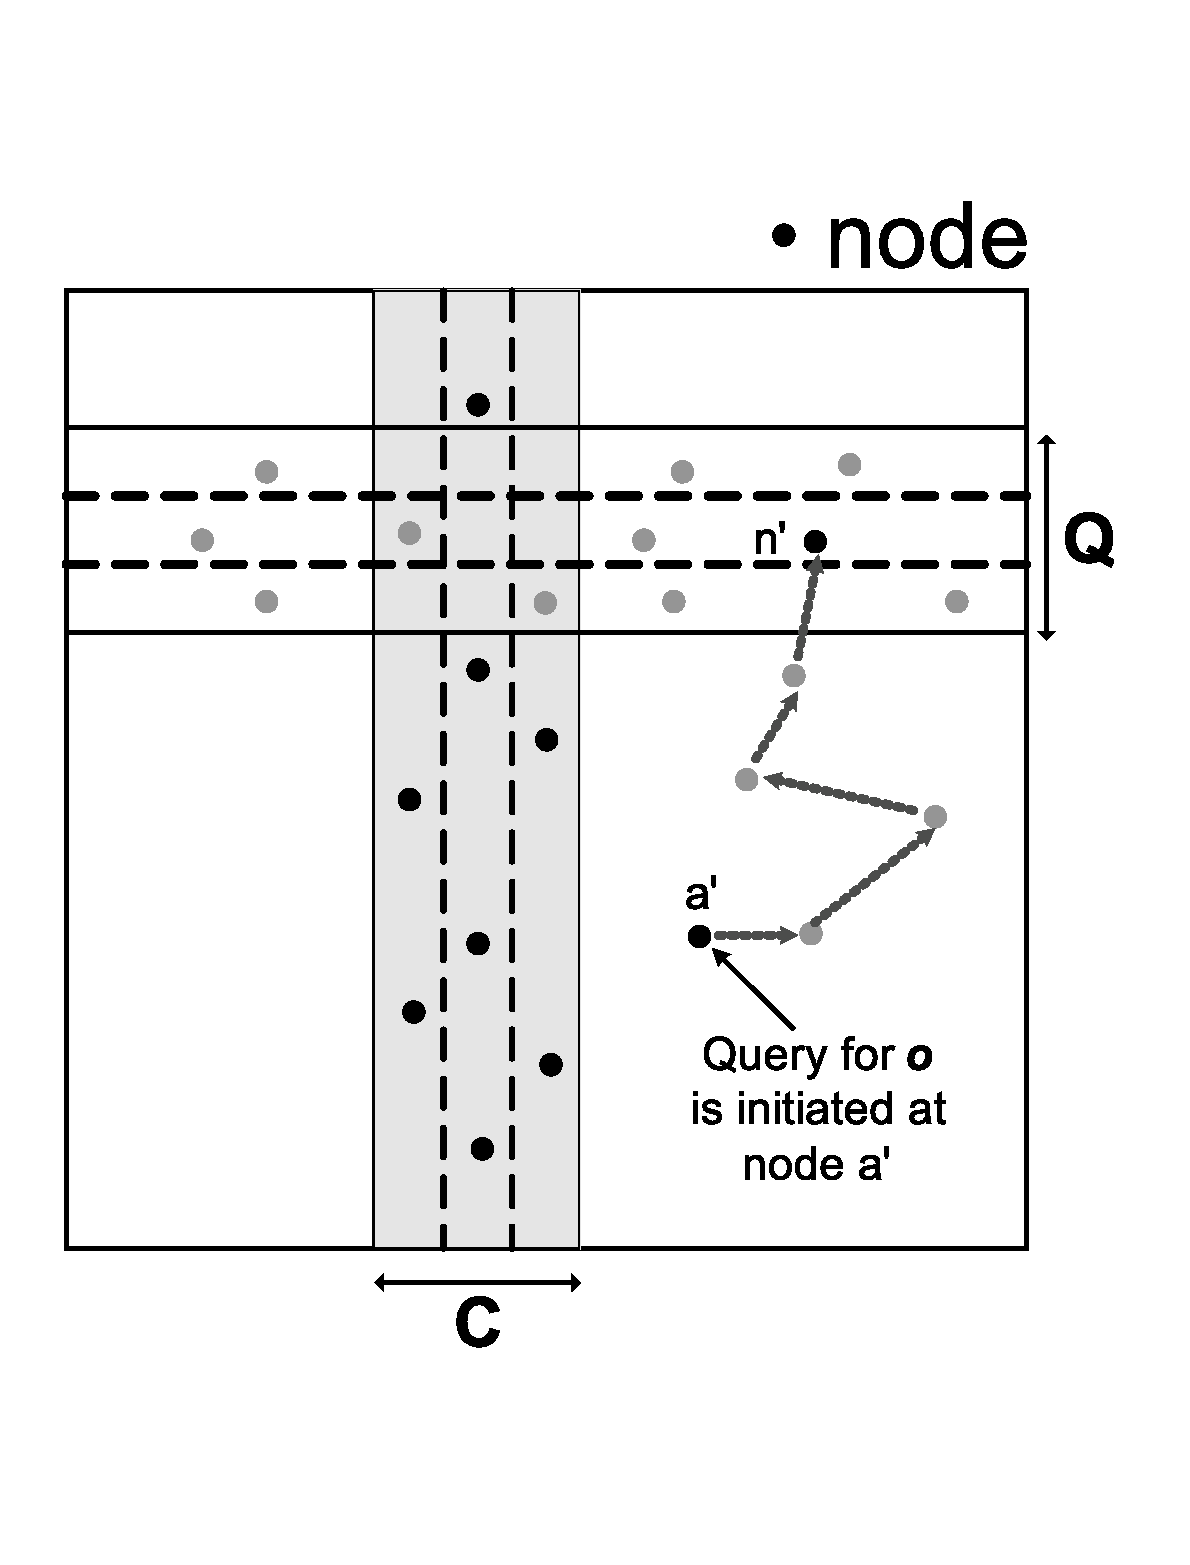
\includegraphics[width=1.4in]{query_1}
\caption{A query for object $o$ is initiated by a node
$a^\prime$.} \label{fig:query1}
\end{minipage}
& \begin{minipage}[t]{2.1in}
\centering
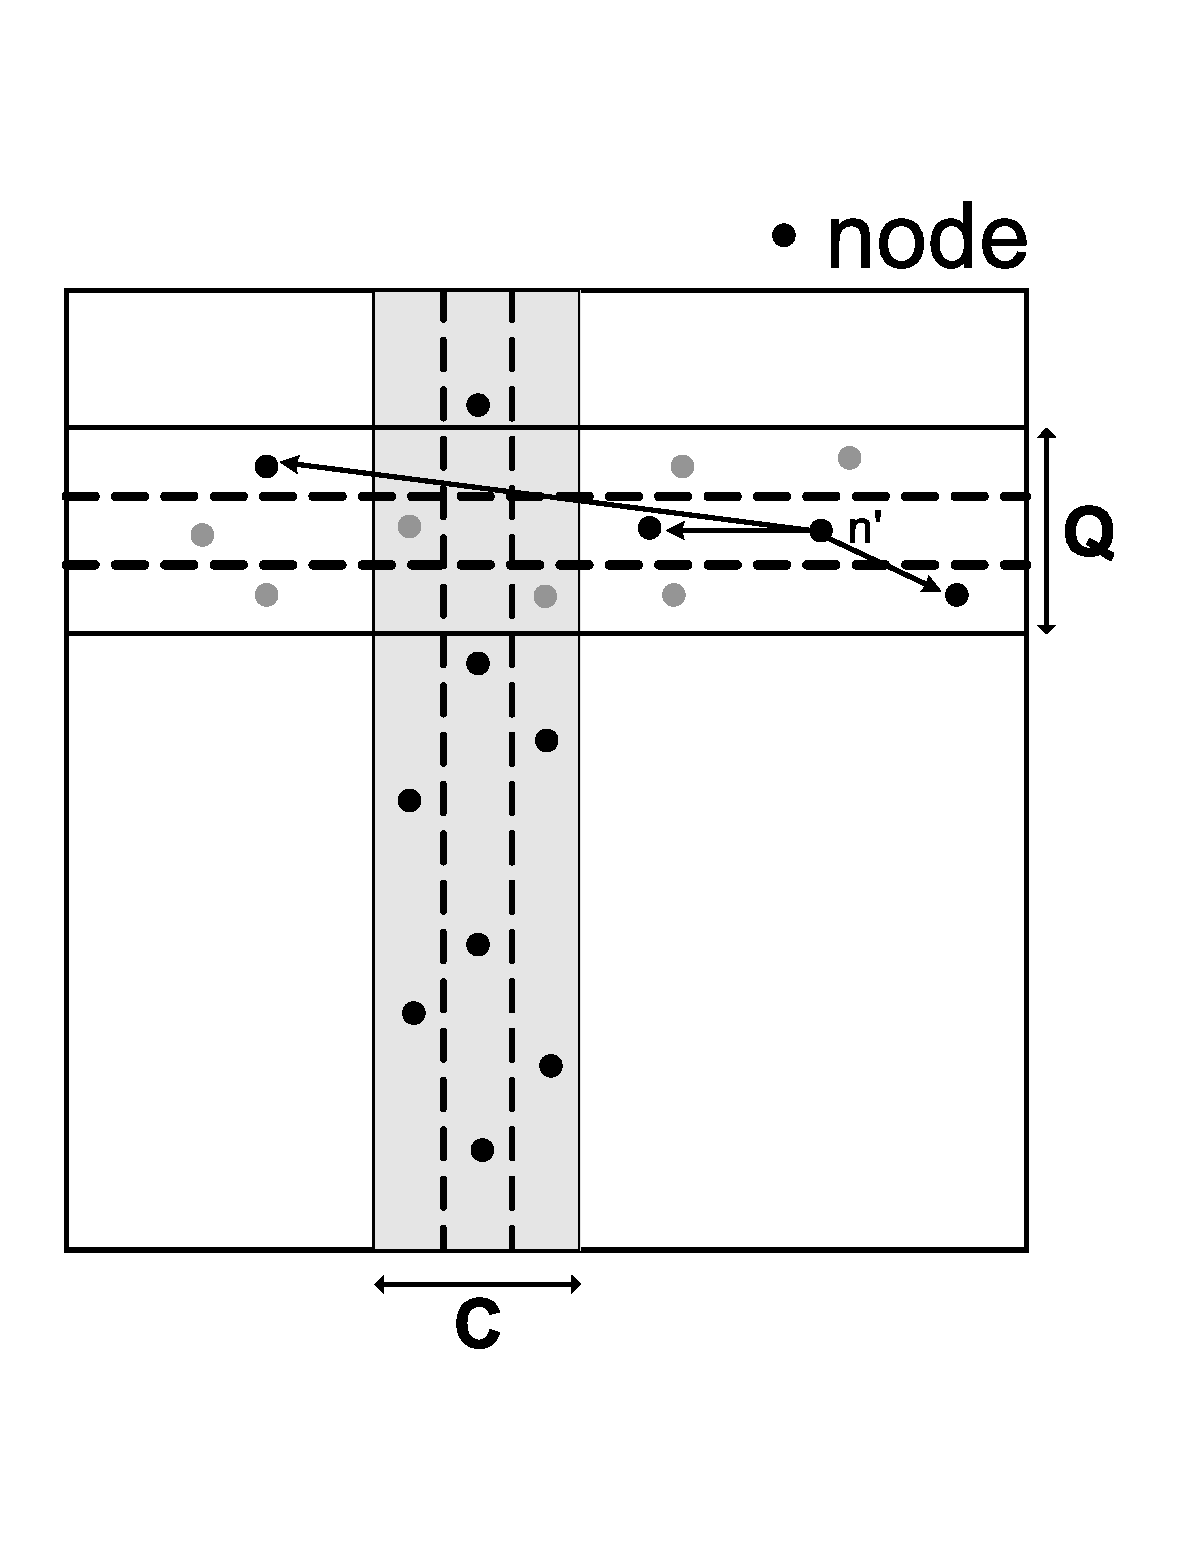
\includegraphics[width=1.4in]{query_2}
\caption{$n^\prime$ starts bounded broadcasting within $Q$}
\label{fig:query2}
\end{minipage}
& \begin{minipage}[t]{2.1in}
\centering
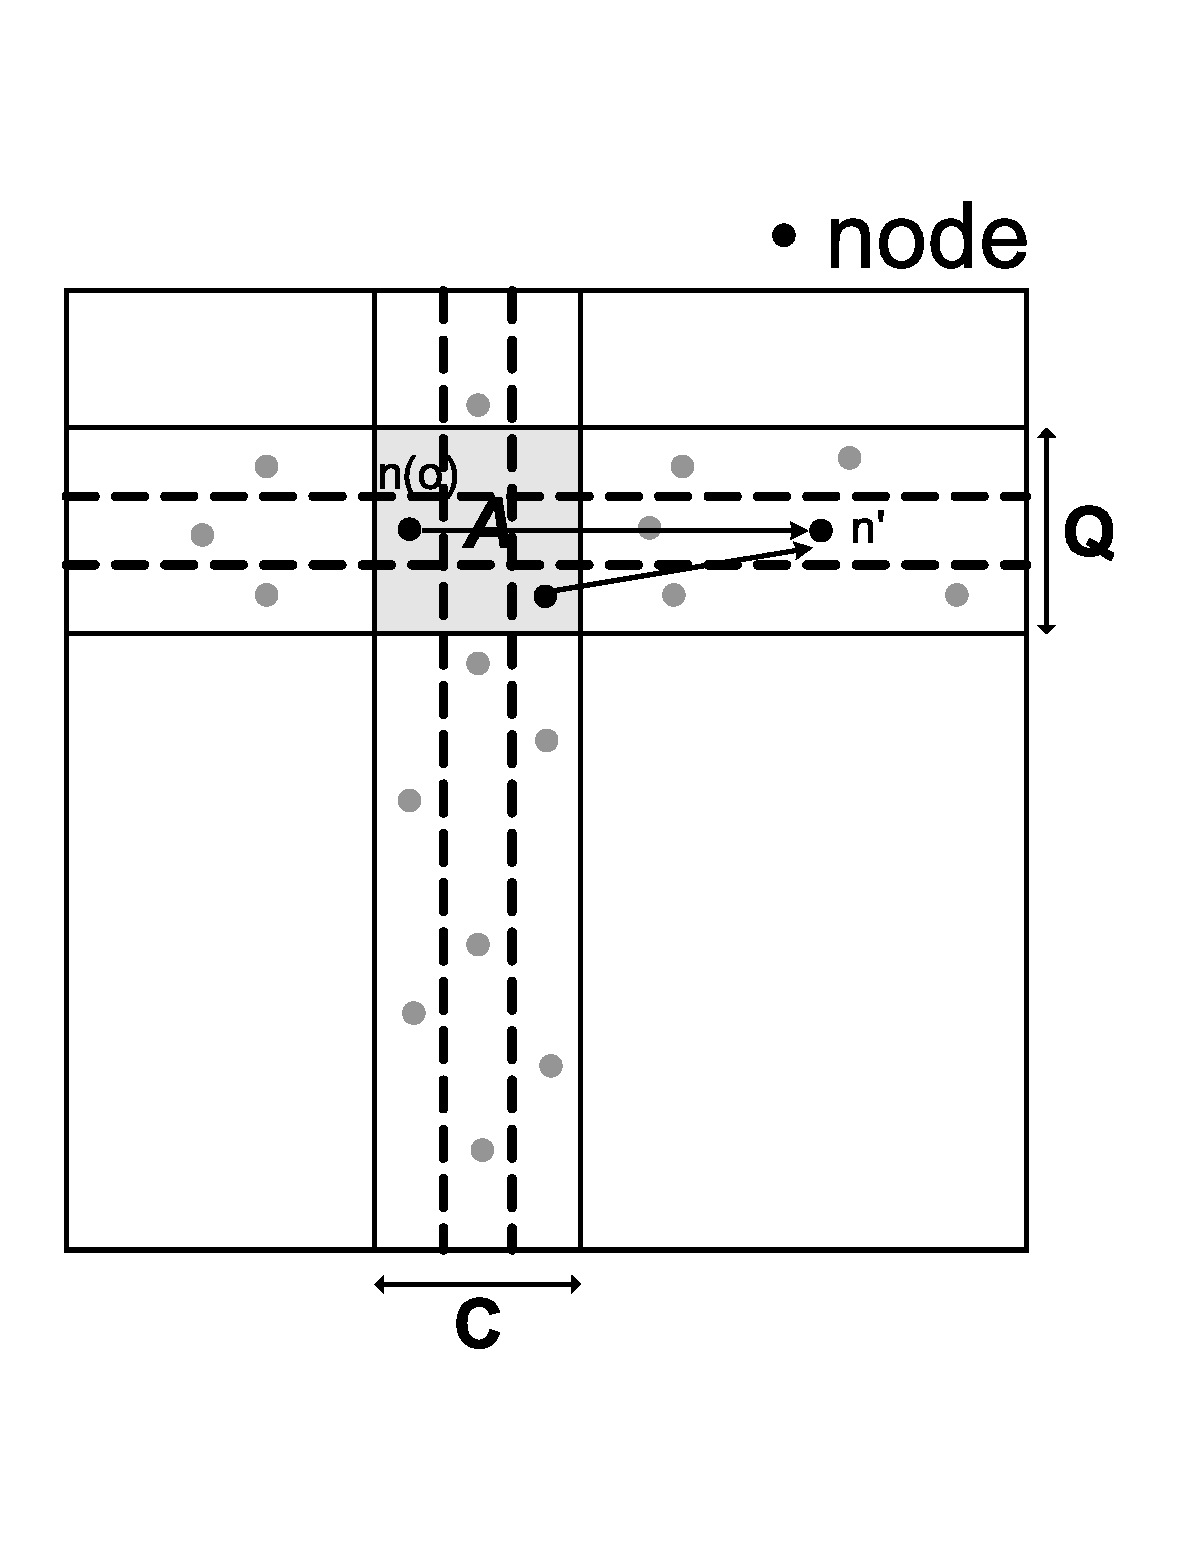
\includegraphics[width=1.4in]{query_3}
\caption{Finally, $n^\prime$ retrieves an object from a node $n(o)$.}
\label{fig:query3}
\end{minipage}\\
\end{tabular}
\end{figure*}
\end{center}

\subsection{Node Joins, Leaves, and Stabilization}\label{sec:join}
In this section, we describe how a node joins and leaves the network. 
Deetoo requires that each data object is cached over the desired 
range in a network. However, a new node joins the network with no cached 
objects. 
Success probability must stay constant regardless of node joins or leaves.
Thus, it is necessary that all objects be replicated 
if a new node's address falls in a object's cached range.
Deetoo relies on a new node copying objects from its new neighbors. 
We define this replicating process as \emph{stabilization} in this paper.

When a new node joins a network, the following steps are taken: 
\begin{enumerate}
%\item select two different random addresses, 
%\item calculate minimum ring distances to neighboring nodes which have 
%      left closest address and right closest address,
%\item find a proper place on the virtual ring space by selecting address 
%      whose minimum distance to neighbor node is bigger than the other,
\item pick a random address
%\item obtain an address and 
\item makes a connection to two adjacent
      neighbors and one short-cut neighbor based on Kleinberg's
      \emph{inverse $r^{th}$-power distribution}, 
\item as a final step, copy objects from neighbors in the same 
      set of sub-rings (in the same columns in matrix space). 
\end{enumerate}
%\begin{figure}
%\centering
%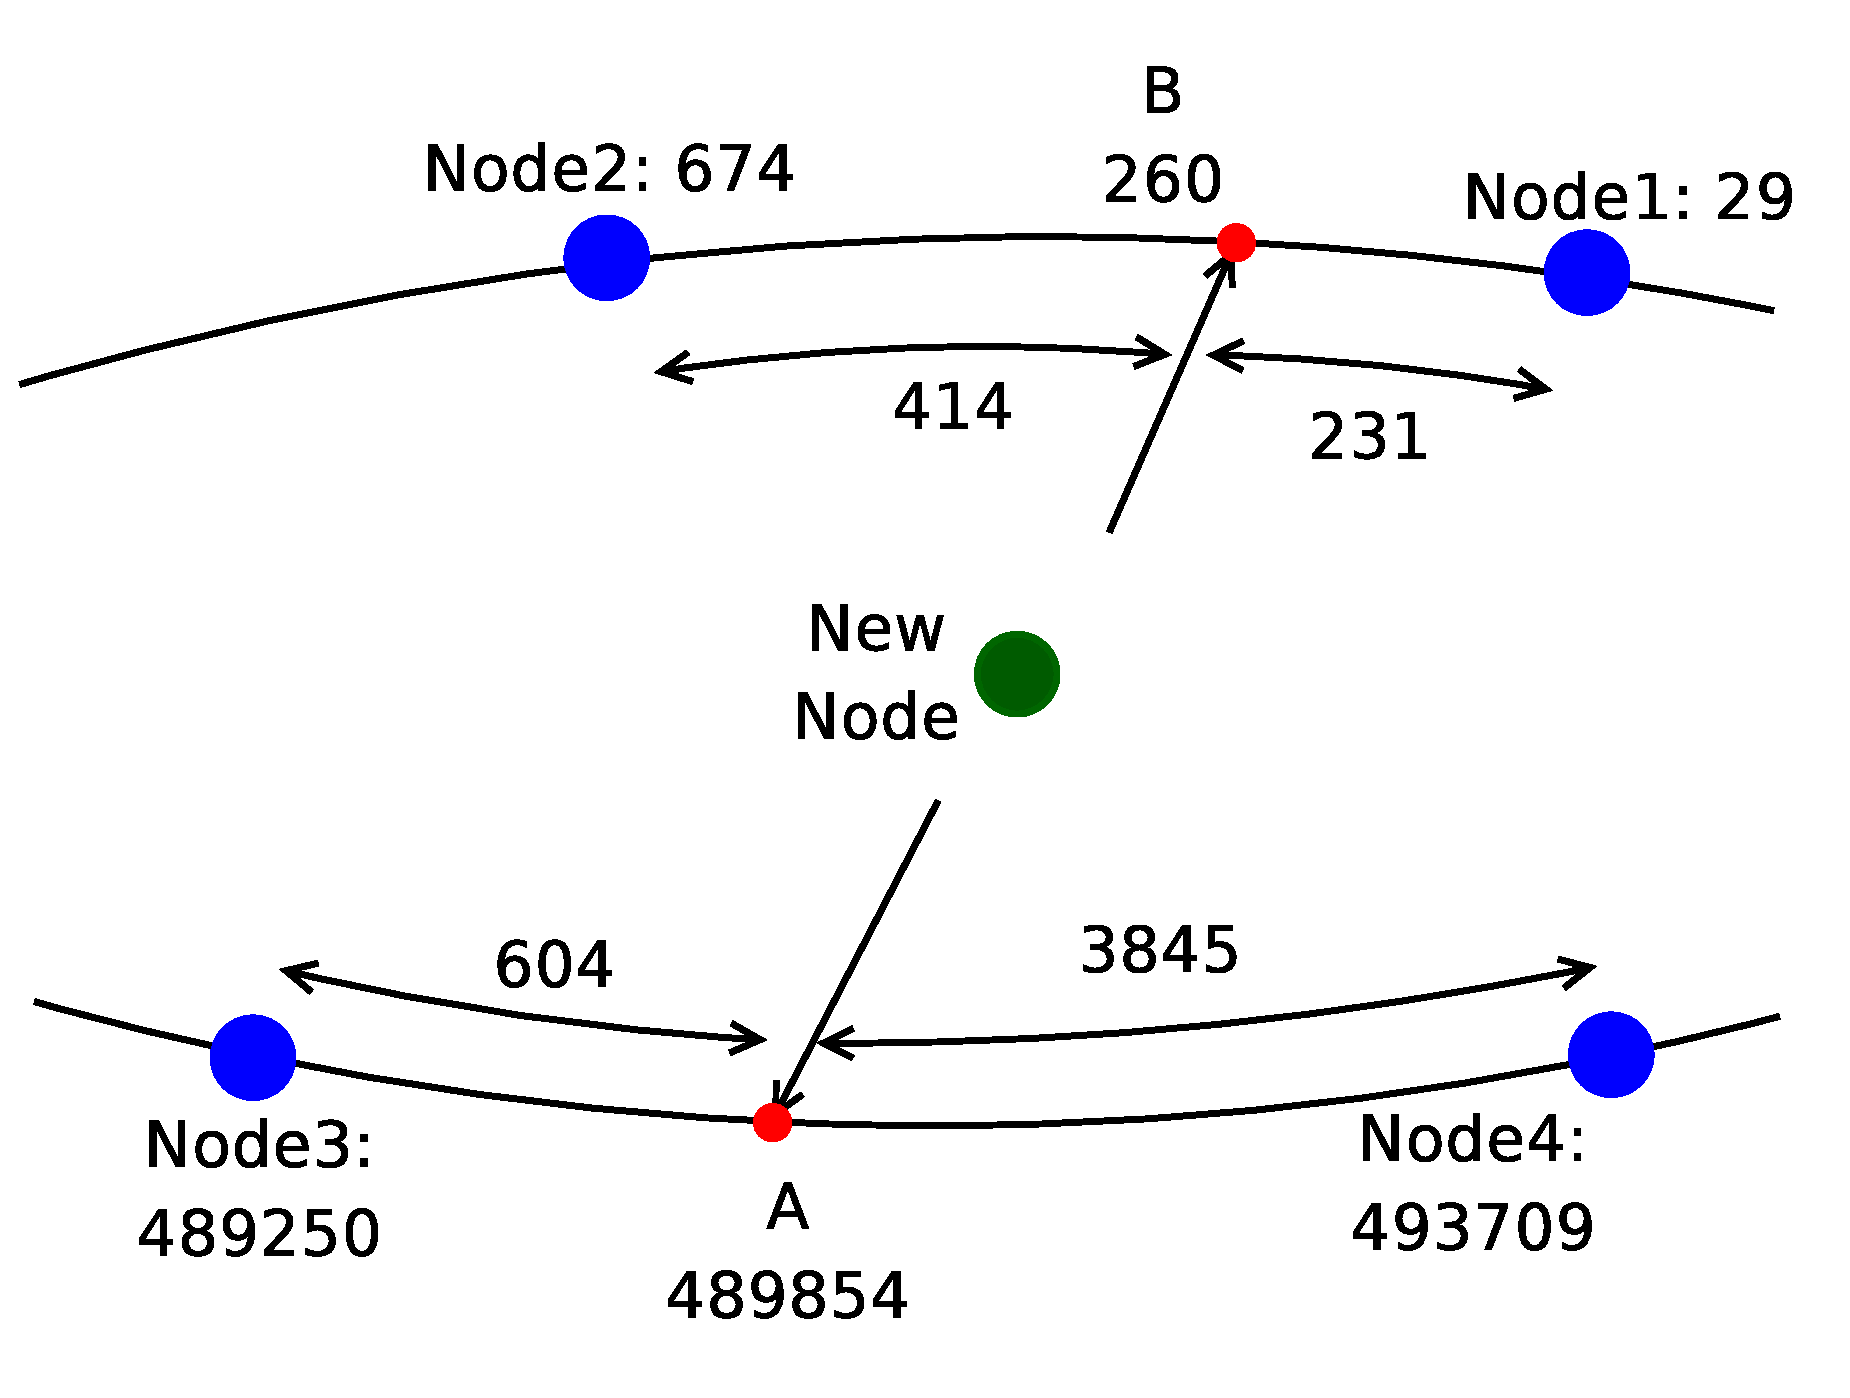
\includegraphics[width=3 in]{evenNet}
%\caption{Choosing a position on the ring when a node joins Deetoo.} \label{fig:join}
%\end{figure}
%Figure \ref{fig:join} shows how a new node finds its right place.
%From randomly selected positions \emph{A} and \emph{B}, the nearest neighbors are 
%\emph{node1} and \emph{node3}. Between these two nodes, 
%\emph{node3} has a bigger distance to \emph{A} than the distance 
%from \emph{node1} to \emph {B}. Thus, a new node takes a position \emph{A} as 
%its new address. 

Each object must keep its range information as well as the object itself or meta data 
for the object where 
it was initially inserted to the network so that as nodes join and
leave the objects can be maintained on their randomly selected column.
% above sentence may need to be modified.
After a node obtains a proper address successfully, the node sends requests to 
its newly connected neighbors in order to replicate objects in the network.  
\emph{Stabilization} plays a role in this stage of replication. 
The following describes how all objects in the same boundary are 
copied to the new successfully joined node from neighbors.
\begin{enumerate}
\item Retrieve the object's range from the neighbor's object list.
\item Recalculate range with a given replication factor.
\item Copy the object from the neighbor node to the 
newly joined node only if the new node's address lies on the recalculated range.
\item Repeat 1 through 3 for all objects from both adjacent neighbors.
\end{enumerate}
If we assume that there exist \emph{k} unique objects in the network whose size is \emph{N}, 
each node maintains $k\frac{\alpha}{\sqrt{N}}$ objects on average, where $\alpha$ is a 
replication factor. In the stage of stabilization, the node is able to receive objects 
from both neighbors. The maximum number of objects which need to be transferred is limited to 
$O(\frac{1}{\sqrt{N}})$.
We analyze \emph{stabilization cost} in Section \ref{sec:stabilization_cost}. 
We also simulate stabilization cost at the time of new node joins 
under churn and compare the simulation result with an analytical model.  
The simulation result shows that Deetoo requires very low stabilization cost. 
When a node leaves or fails, our protocol
does not need to do anything because all objects have already been copied to
all nodes in the same set of columns. Thus, neighbor nodes keep exactly
the copies of the objects held by leaving or failing nodes.

\iffalse
\subsection{Estimating Network Size}
Each node in a Deetoo network is distributed without any 
server-client interaction, which makes it impossible for the peers to know exactly how many other peers 
exist. However, each node is required to know the network size in certain processes. 
For example, we cannot decide a caching or a 
querying size without knowing the number of peers in the network.
The accuracy of network size estimation is key to deciding the optimal 
caching and querying range. 
Both underestimation and overestimation 
affect performance in success probability and communication cost. 
If a node underestimates the size of the network, 
the success probability goes down below average while the communication 
cost is reduced. The exact opposite result is expected if a bigger size 
is estimated. 

Deetoo introduces two methods to reduce network size estimation error. 
The first method is that Deetoo helps a newly joining node finding a 
right place. In the previous section, we explained 
how a node selects a new address between two candidates. 
Although choosing a random address is much simpler than our method, 
our method makes distances between every two nodes more evenly distributed 
because it always maximizes the minimum distance between two adjacent nodes. 
As a result, the variance of distance distribution between two nodes is reduced.  
Next, the average distance between nodes is estimated using a multi-hop-away node. 
To utilize this approach, we divided this process into two steps. 
First, the distance between two direct neighbors is calculated 
to get the initial guess for a network size, $N_0$.
Let an address have $b$ bits; then the whole address space is B=$2^{b}$, which
is equal to ring distance $D_{ring}$.  Node $n$ calculates the 
average distance to its neighbors ($D_0$). Then, the first
network size, $N_0$($\simeq$ $\frac{B}{D_0}$) is estimated. 
Second, the average distance, $D_1$, from $n$ to a node 
which is $\log N_0$ hops away from $n$ is counted. The final network size 
estimated, $N_{est}$($\simeq \frac{B}{D_1}$) can be evaluated.
We experimented under various settings to get the best estimation 
of the network size. If more nodes are involved in calculating the average 
distance between two nodes, the level of accuracy goes up though it requires 
more time and bandwidth. On the contrary, the variance of the average distance 
is much higher when only two direct neighbors are used for the calculation. 
We lose accuracy of size estimation in this case though we save 
time and bandwidth.
We observed that our calculation of the average distance using $\log N$ 
hops is acceptable considering both accuracy and cost. 
Figure \ref{fig:histogram} shows estimated network size distribution under our 
network size estimating algorithm. 
In Figure \ref{fig:anal}, the simulation results show that our network 
size estimation works well in that the success probability is very close to 
the theoretical expectation.

\begin{center}
\begin{figure*}[ht]
\centering
\begin{tabular}{c c}
\begin{minipage}[t]{3in}
\centering
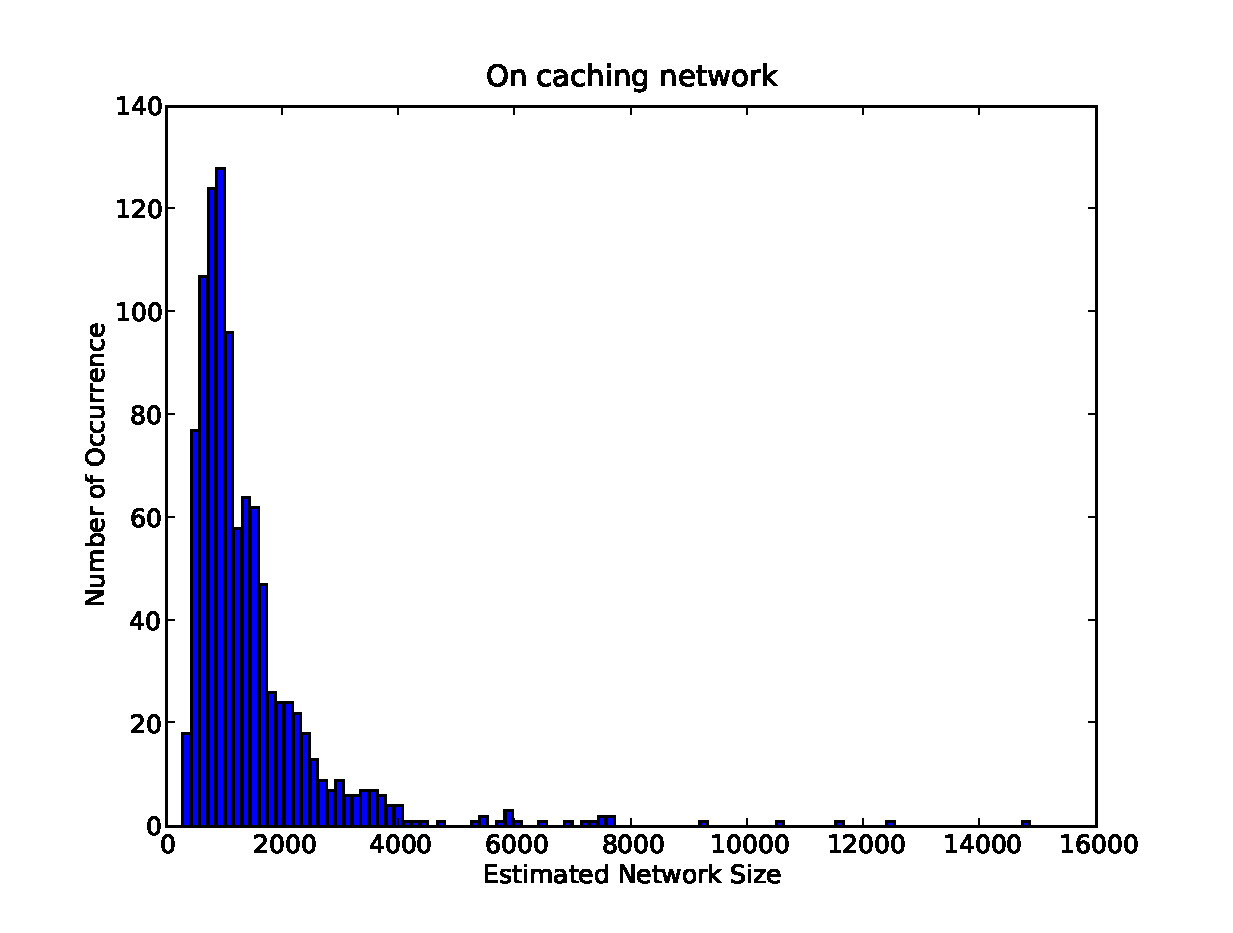
\includegraphics[width=2.5in]{hist_c}
\end{minipage}
& \begin{minipage}[t]{3in}
\centering
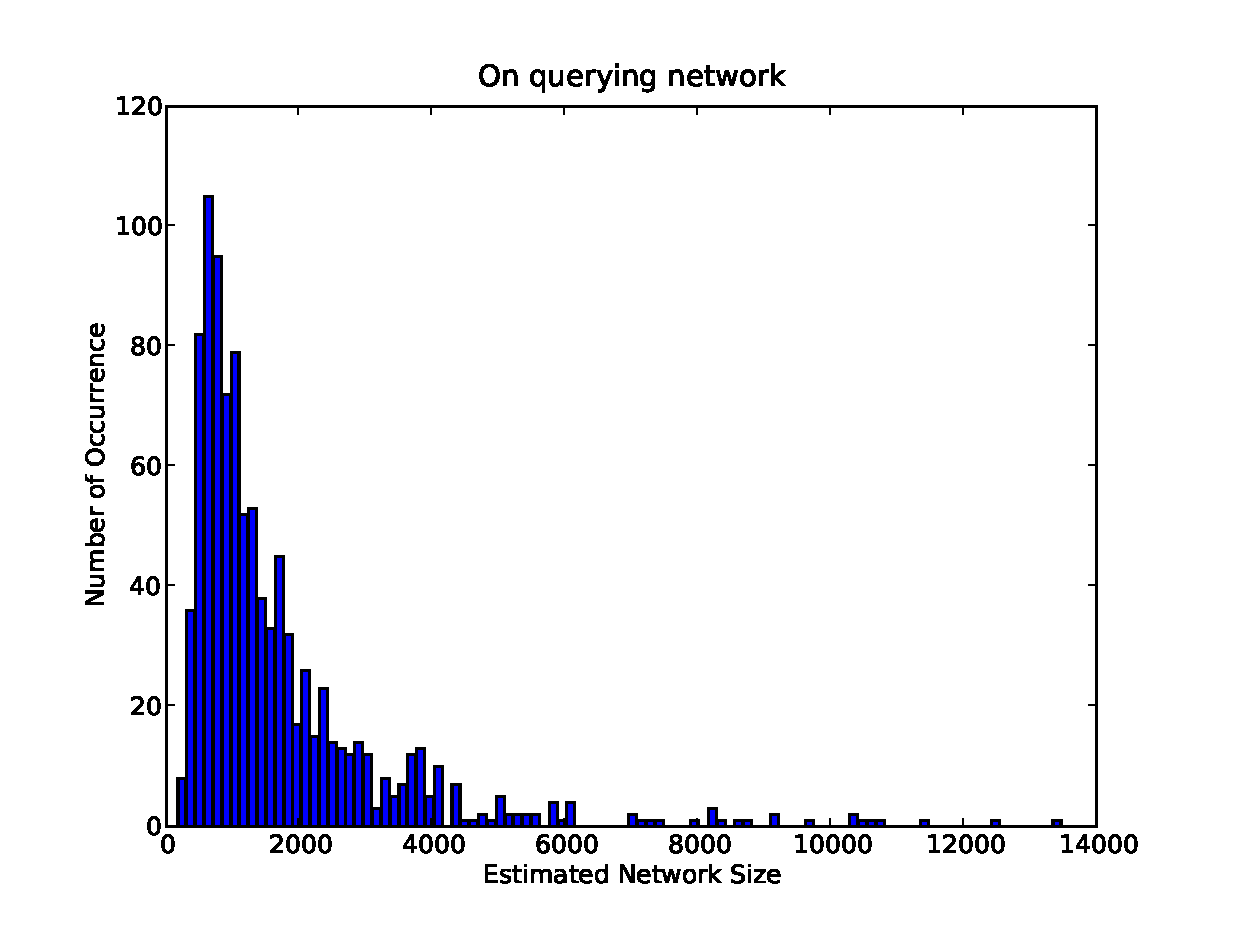
\includegraphics[width=2.5in]{hist_q}
\end{minipage}\\
\end{tabular}
\caption{Estimation size distribution. The actual network size is 1,000. 
The averages are 1430.97 and 1695.95 for caching and querying, respectively.
The standard deviations are 1248.56 and 1630.41, respectively.
The medians are 1077 and 1144, respectively. Note that the error margin 
of overestimation is much larger than that of underestimation, which causes
the average to be slightly larger than the actual size of network. 
Network size estimation for cache is more accurate than that for query, 
because new node's address selection is based on caching address.} 

\label{fig:histogram}
\end{figure*}
\end{center}
\fi

\section{Analysis of Deetoo}\label{sec:analysis}
Our analysis focuses on the probability of a query being successfully resolved
, $P_{s}$, and the communication cost, $K$, 
to show that the Deetoo protocol for unstructured P2P
networks is efficient and scalable. We build the following assumptions to 
simplify our analytical modeling.
First, we have a fixed size of the addresses. Thus
address space, $B$, is fixed, which is $m$ $\times$
$m$ for cache and query respectively as shown in
Figure \ref{fig:space}. Second, we assume that the caching probability we
cache at location $i$, $c_{i}$, and the querying
probability we put a query at location $j$, $q_{j}$, are both
uniformly distributed. Third, we assume that the caching and querying
probability are the same at any location. Finally, at most one node per
a bin in matrix space is allowed for all nodes to have a unique
address.
%Our analysis and simulation about search hit consider only 
%exact matching search. 


\subsection{Success Probability}
\label{sec:suc_prob}
We define the success probability, $P_{s}$, to be the probability
that an answer to the query is found. Assume that each vertex in the
matrix space has a node with probability $p$. The probability
we can not successfully resolve a query is the product of probability that no
node in the overlapping area between caching space and querying
space. It is not hard to see that:
\begin{center}
\begin{eqnarray*}
1-P_{s} = \prod_{A}(1-p) = (1-p)^{C Q}
\end{eqnarray*}
\end{center}
because area \textit{A} has $C\times Q$ bins.
The expected number of the nodes in the whole space, 
$N$, equals to $pB$. Thus, $p = \frac{N}{B}$.
We set $C\times Q = \alpha \frac{B}{N}$,
which can be achieved with very high probability because we assumed
that nodes are distributed uniformly in the matrix (lattice) space.
One column or row has $\sqrt{N}$ nodes with very high probability
and its address space has size of $\sqrt{B}$. 

\begin{eqnarray*}%\label{th}
1-P_{s} &=& \left(1-\frac{N}{B}\right)^{\alpha \frac{B}{N}}\\
        &\le& e^{-\alpha}\\
	P_{s} &\ge & 1 - e^{-\alpha}
\end{eqnarray*} 
The above bound is tight when $\frac{N}{B}\rightarrow 0$,
which is the case of a sparse address space (much fewer nodes 
than bins).
So, we are able to have success probability solely as a function of the 
constant replication factor $\alpha$, and totally 
independent of the number of the nodes.

\subsection{Communication cost}
In order to check the network's scalability, communication costs
need to be examined. Each caching message is transferred to all the
nodes in the shaded area in Figure \ref{fig:cache3}, and this area has
$C\sqrt{B}$ bins. Since we assume that cache and query probabilities are
equal, $C = Q = \sqrt{\alpha B/N}$; therefore either caching cost or querying cost $K$ is:
\begin{eqnarray*}\label{th}
K &=& pC\sqrt{B} \  (\mathrm{or}\  pQ\sqrt{B})\\
  &=& \frac{N}{B}C\sqrt{B} = \frac{N}{B}\sqrt{\frac{\alpha B}{N}}\sqrt{B}\\
  &=& \sqrt{\alpha N}
\end{eqnarray*}
From the above analysis, we show that a query in the network
generates $O(\sqrt{N})$ messages.

\subsection{Search time}
\label{sec:search_time}
Search time can be analyzed by computing the average
depth of the tree formed by the bounded broadcast presented in
Section \ref{sec:broadcast}. When we assume that each node 
has a connection to its nearest neighbors on both rings as well as
one shortcut connection to a node at distance $d$ with probability
proportional to $1/d$, we can show that the expected depth of the 
tree is $O(\log^2 N)$. 
Our proof is analogous to computing the average time 
to reach a node using greedy routing as in \cite{jk:Information,
pr:Symphony}, while search time of 
Deetoo measures the average maximum depth of the local trees.
\begin{figure}
\centering
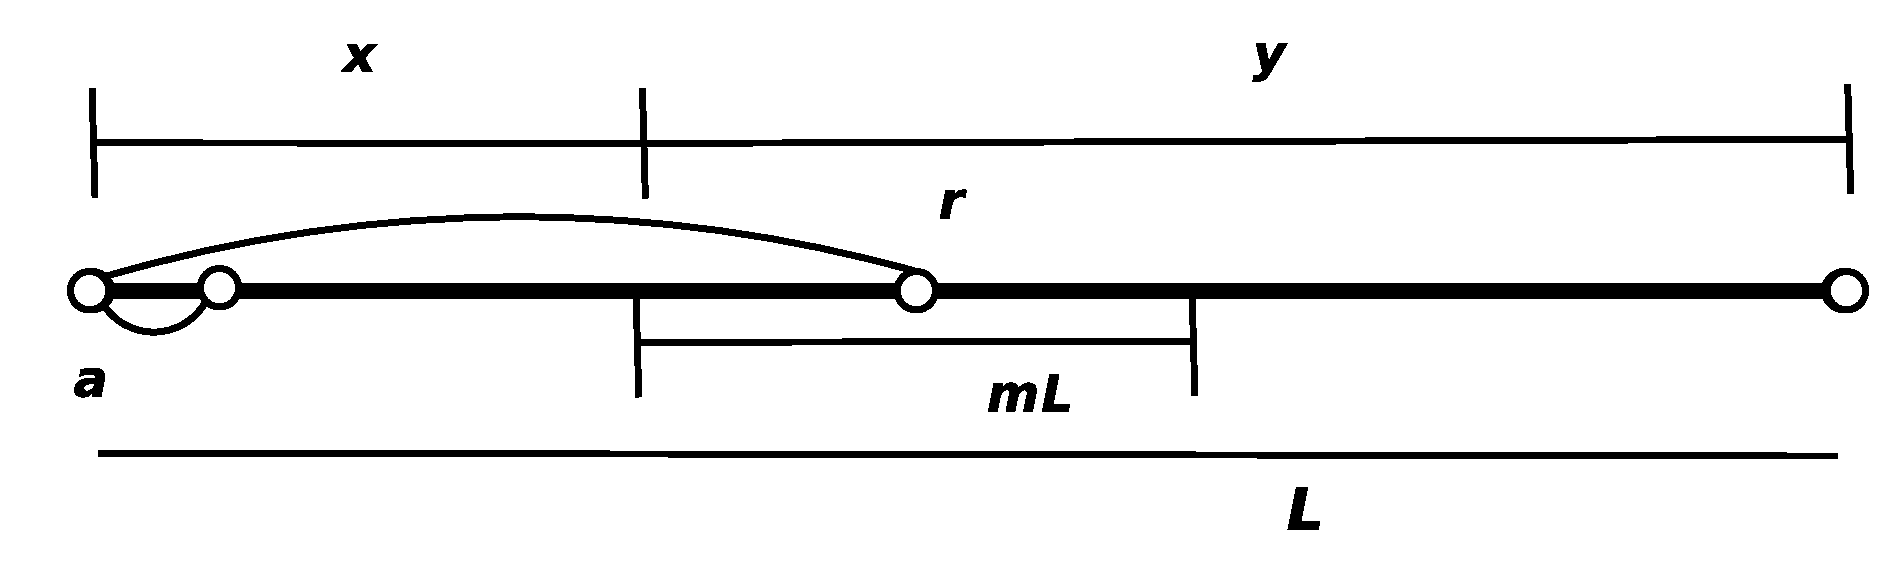
\includegraphics[width=3 in]{searchtime}
\caption{The probability that a node \textit{a} has a connection to a node \textit{r} 
in the middle(region \textit{mL}) is defined as $p_{m}$, and $p_m$ is inverse 
proportional to the distance between \textit{a} and \textit{r}.} \label{fig:search}
\end{figure}
From the Kleinberg's model, each node has a long-range
contact at distance \textit{r} with probability 
$p_{r}=\frac{1}{\log N}\frac{1}{r}$ as in Figure \ref{fig:search}. 
Let \textit{$p_{m}$} be the probability that node \textit{a} has a long-range
contact in the middle, \textit{$mL$} region.
\begin{eqnarray*}
p_{m} &=& \sum_{r=\frac{1-m}{2}L}^{\frac{1+m}{2}L}p_{r}\\
        &=& \sum_{r=\frac{1-m}{2}L}^{\frac{1+m}{2}L}\frac{1}{\log
        N}\frac{1}{r}\\
        &\simeq& \frac{1}{\log N}\log\left(\frac{1+m}{1-m}\right)
\end{eqnarray*}
Since \textit{$mL$} is a subset of \textit{$L$},
$m\in (0,1)$. 
Let $T(i)$ be the search time in region of size $i$.
Each long range connection either goes to a node in the
middle region or not.
If we make it into the middle region, the remaining area
to search is at most the length of $\frac{1}{2}L + \frac{m}{2}L$.
Thus,
if the long-range connection goes to the middle, the time is 
$T(L) \leq 1 + T((\frac{1+m}{2})L)$. 
Otherwise, we go to the next neighbor so $T(L) = 1 + T(L-1)$.
We know that $T(L-1) < T(L)$.  If $p_m$ is the probability of making
it into the middle, on average, we need to try $1/p_m$ neighbors before
we are likely to find a connection to the middle.  Putting this together,
the average search time is
$T(L) \leq \frac{1}{p_m} + T((\frac{1+m}{2})L)$. 
The first part of the right side of the equation represents time to reach 
a connection in the middle (\textit{x} in Figure \ref{fig:search}) and 
the second part is time for the rest of the region (\textit{y} in Figure \ref{fig:search}. 
For the rest of the region, at most $\gamma$ more steps are required to 
cover the whole region \textit{L}. We know $T(\log{N}) \leq \log N$. 
Solving for $\gamma$ such that $(\frac{1+m}{2})^{\gamma}L = \log N$, 
\begin{eqnarray*}
\gamma \leq \frac{\frac{1}{2}\log{(\alpha N})}{\log{(\frac{1+m}{2})}}
\end{eqnarray*}
The maximum depth is decided to $\gamma$ steps multiplied by the number of the nodes 
to reach a connection in the middle.
\begin{eqnarray*}
T(L) &\leq& \frac{1}{p_m}\gamma \\
     &=& \frac{\log N}{\log{(\frac{1+m}{1-m})}}\frac{\frac{1}{2}\log{(\alpha N)}}{\log{(\frac{1+m}{2})}}
 \\
     &\leq& \frac{\frac{1}{2}(\log^2 (\alpha N)-\log{\alpha}\log{(\alpha N))}}{\log{(\frac{1+m}{1-m})}\log{(\frac{1+m}{2})}}
\end{eqnarray*}
We calculate an upper bound with the above inequality by getting the maximum 
of the denominator.
At a value of $m\approx0.517$, the denominator of the right side of the above inequality has a minimum. 
In consequence, the upper bound for $T(L)$ is minimized.
We verify this claim using simulations which are presented in Figure \ref{fig:time}. 
For the comparison, the minimum of upper bound, where \textit{m} is set to 0.5, is 
calculated and compared with our simulation result.

\subsection{Stabilization Cost}
\label{sec:stabilization_cost}
We regard the number of objects that need to be copied to 
a newly joined node as the stabilization cost 
because there is no other major message transmission 
except this copying for a leaving or joining node. 
We assume that our algorithm checks whether an object 
is already replicated from either neighbor or not. If a node identifies the 
object, it discontinues the object transmission. This ensures that a node 
prevents unnecessary message generation and a network saves bandwidth.
Objects which already exist in a new node as well as out of 
object's range are excluded from transmission.
A new node examines each object's range whenever it is ready to be copied.
In P2P networks, network size often varies. Thus, as the network
size changes, the object's range is recalculated.
Caching in a redefined range constrains the number of 
cached replicas to remain $O(\sqrt{N})$.
 
Let $C_s$ represent the stabilization cost, $k$ the number of unique objects in the network, 
$N_1$ the left neighbor, 
and $N_2$ the right neighbor. Let $\eta_i$ symbolize a probability of the object in node $N_i$. 
$\eta_{ij}$ is a probability of the object in both $N_i$ and $N_j$ and  
$\eta_{j|i}$ denotes a probability of the object in $N_j$ given that the object is in 
$N_i$. 
\begin{eqnarray*}
C_s &=& k P(object\ in\ N_1\ or\ N_2) \\
    &=& k (P(object\ in\ N_1)+P(object\ in\ N_2)\\
    &&-P(object\ in\ both\ N_1\ and\ N_2)  \\
    &=& k (\eta_1+\eta_2-\eta_{12}) \\
    &=& k (\eta_1+\eta_2-\eta_1\eta_{2|1})
\end{eqnarray*}
The probabilities, $\eta_i$ and $\eta_{ij}$, are calculated as follows:
\begin{eqnarray*}
\eta_1 &=& \eta_2 = \frac{L}{B} \\
       &=& \frac{\sqrt{\alpha N} d_{ave} }{d_{ave} N} \\
       &=& \sqrt{\frac{\alpha}{N}} \\
\eta_{12} &=& \eta_1 \eta_{2|1} \\
          &=& \sqrt{\frac{\alpha}{N}}\left( 1-\frac{d_{ave}}{L} \right) \\
          &=& \sqrt{\frac{\alpha}{N}}\left(1-\frac{1}{\sqrt{\alpha N}}\right) \\
\end{eqnarray*}
Thus,
\begin{eqnarray*}
C_s &=& k\left(2\sqrt{\frac{\alpha}{N}}-\sqrt{\frac{\alpha}{N}}\left(1-\frac{1}{\sqrt{\alpha N}}\right) \right) \\
    &=& k(\sqrt{\frac{\alpha}{N}}+\frac{1}{N}) \\
    &=& O\left(k\sqrt{\frac{\alpha}{N}}\right)
\end{eqnarray*}
where $d_{ave}$ denotes the average distance between two nodes, 
$N$, $B$, and $L$ represent the number 
of nodes, the ring distance (the average distance times total number of nodes), 
and the length of bounded broadcasting range (the average distance times the number of 
nodes in the range), respectively.
%Since $L = \sqrt{\alpha N}d_{ave}$ and $B = d_{ave}N$, 

\section{Simulation Results}\label{sec:simulation}
In this section, we confirm the theoretical results discussed in the previous 
section via simulations. 
%tw: elaborate on the simulator
We used Netmodeler\footnote{Netmodeler is a free software/open source
C++ library developed by the authors} for simulating the Deetoo algorithm.
In our topology model on top of Netmodeler, 
each bin may be occupied by at most one node and the nodes form two rings,
one for the cache and the other for query.
\iffalse
% POB: anonymized version of the above
We used a program we developed in C++ for simulating the Deetoo algorithm.
In our topology model, 
each bin may be occupied by at most one node and the nodes form two rings,
one for the cache and the other for query.
\fi
%
Then, each node is connected to a long-range neighbor according
to the \emph{inverse $r^{th}$-power distribution} for the small-world network model. 
For simplicity, the size of the query range is assumed to be the same as the size of the cache 
range. All caching and querying processes are initiated on randomly selected nodes and
messages are broadcasted within randomly chosen ranges.
Network size determines the range of bounded broadcasting for both caching and querying, and
success probabilities and communication costs depend on the accuracy of estimation.
In simulation, the number of nodes in the whole network is estimated by calculating node density
as described in \cite{LuoQHC08}. 
%The analysis of trade-off between accuracy and cost will be analyzed as future work.

\subsection{Performance Evaluation} 
\begin{figure}
\centering
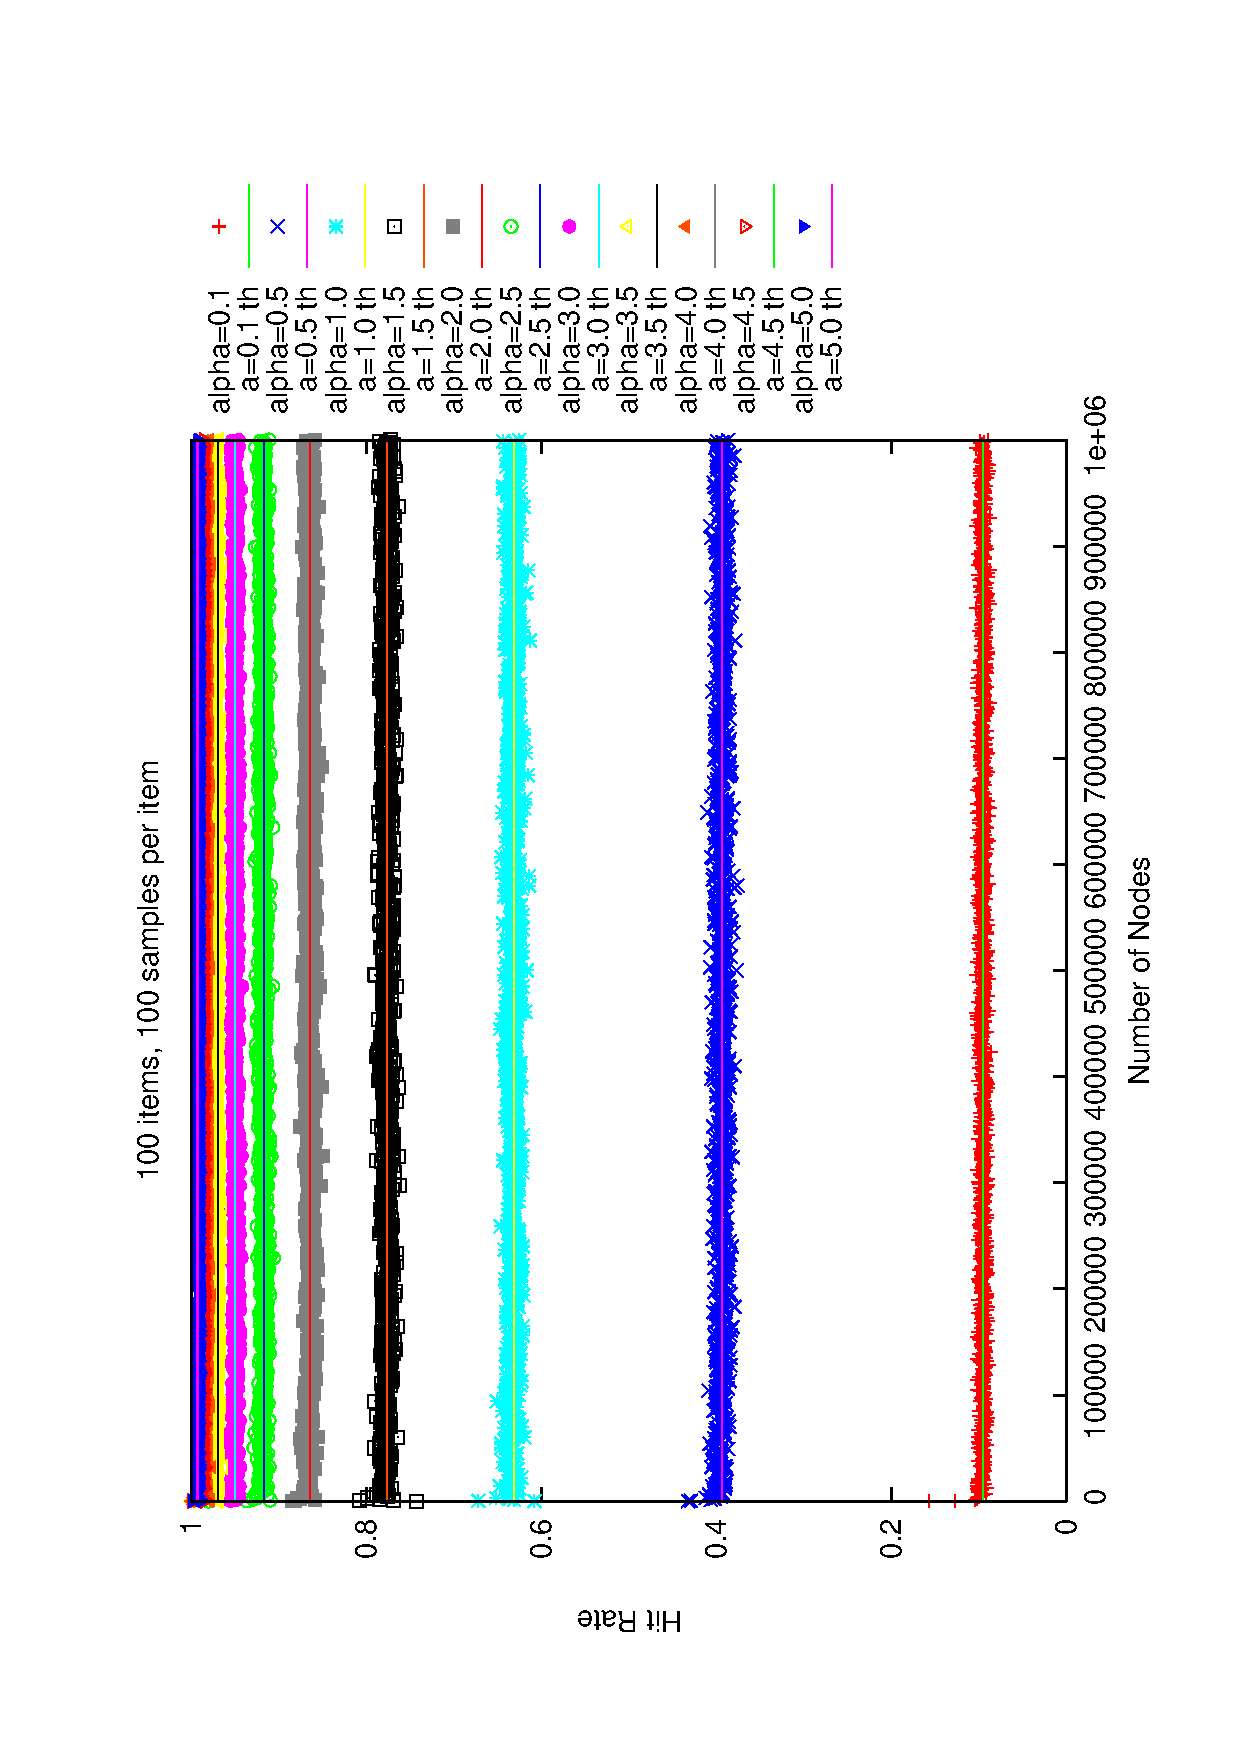
\includegraphics[angle=270,width=3.5in]{th_hitrate}
\caption{Query hit rate is constant in network size $N$, and scales
as $1-e^{-\alpha}$.In the legend, ``th" is theory, the other is simulated.} \label{fig:hitrate}
\end{figure}
\begin{figure}[h]
\centering
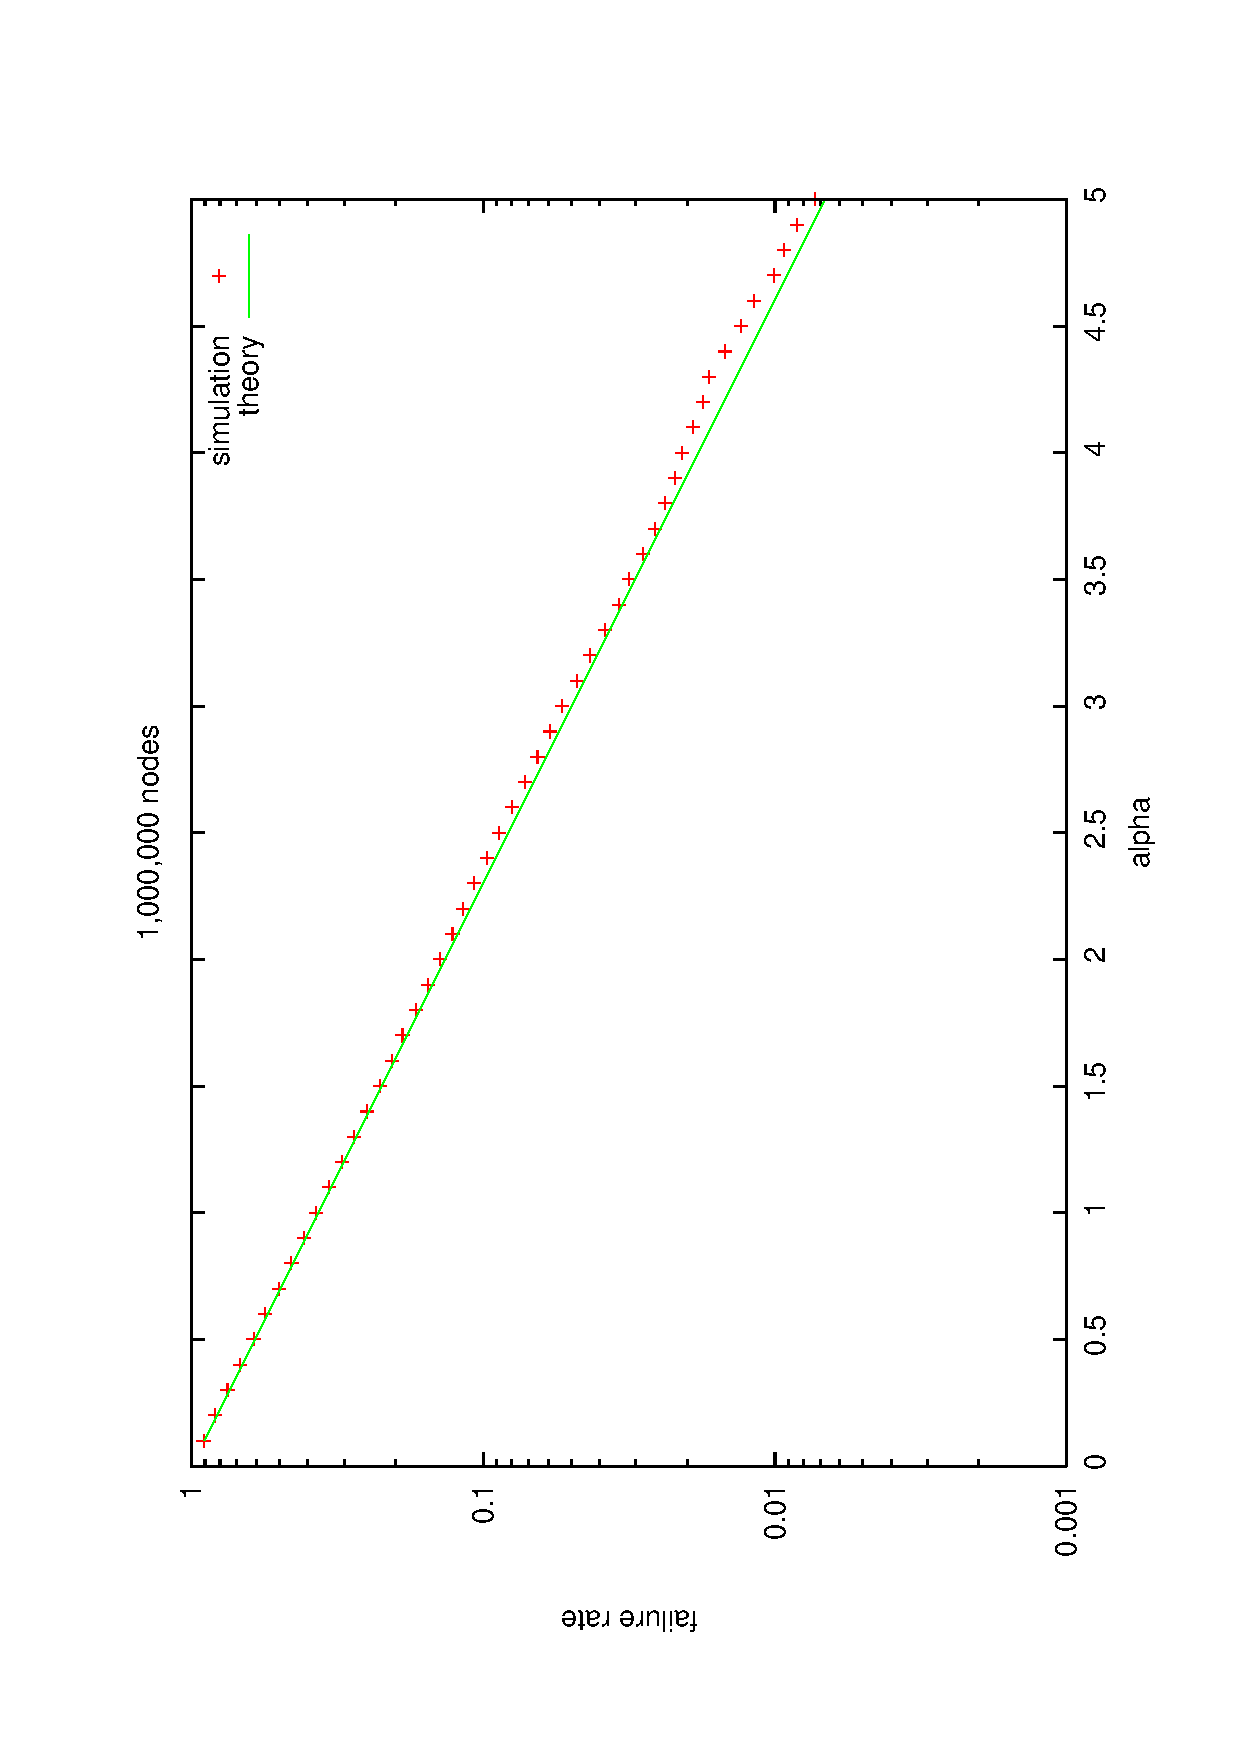
\includegraphics[angle=270, width=3.5in]{mishit_logy}
\caption{Query miss rate as a function of $\alpha$, this scales
as $\exp(-\alpha)$.} \label{fig:mishit}
\end{figure}
In our simulations the size of the address space is set to 32 bits which has $2^{32}$
bins. 
We count the number of hops as an indication of communication cost and assume that the 
per-hop communication costs for cache and query are the same. 
Our simulations are performed on networks of size 10 to $10^{6}$.
The number of columns, $C$, is chosen such that $C$ is equal to the number of rows, $Q$, 
$C^2$ = $\alpha N$. Thus, we simulate various values of $\alpha$ to observe the effect of
increasing or decreasing the cache or query range size ($\alpha$=$\frac{C^2}{N}$). 
We performed simulations with $\alpha$=0.1 to 5.0, with intermediate steps of size 0.1.
100 string objects were generated by using a random string generator.
Each object was initially inserted on a uniformly randomly selected
node.
For queries, we count only exact matching objects even though Deetoo can perform partial matches.
Each test was repeated 100 times and the results were averaged. 
Figure \ref{fig:hitrate} shows that query success probability is constant regardless of 
the network size. The constant success rate is desirable since 
Deetoo can perform the search with preferred success probability by adjusting 
broadcasting range with different $\alpha$.  
In the figure, we also compare the simulation results with the theoretical results.
We observe that the larger the $\alpha$ is, the higher the success probability is.
In Figure \ref{fig:mishit}, query success probability declines exponentially as expected.
% POB: we are deleting this because we don't understand it very well. 
%Relatively high deviation is witnessed with large $\alpha$. Because we estimated success
%probability by assuming $\frac{N}{B} \ll$ 1, it is expected to have
%higher deviation in the case where $N\approx B$.
%
%communication cost (hops)
Figure \ref{fig:cost} shows communication cost with respect to network size. There is 
a trade-off between success probability and the communication cost. 
\begin{figure}
\centering
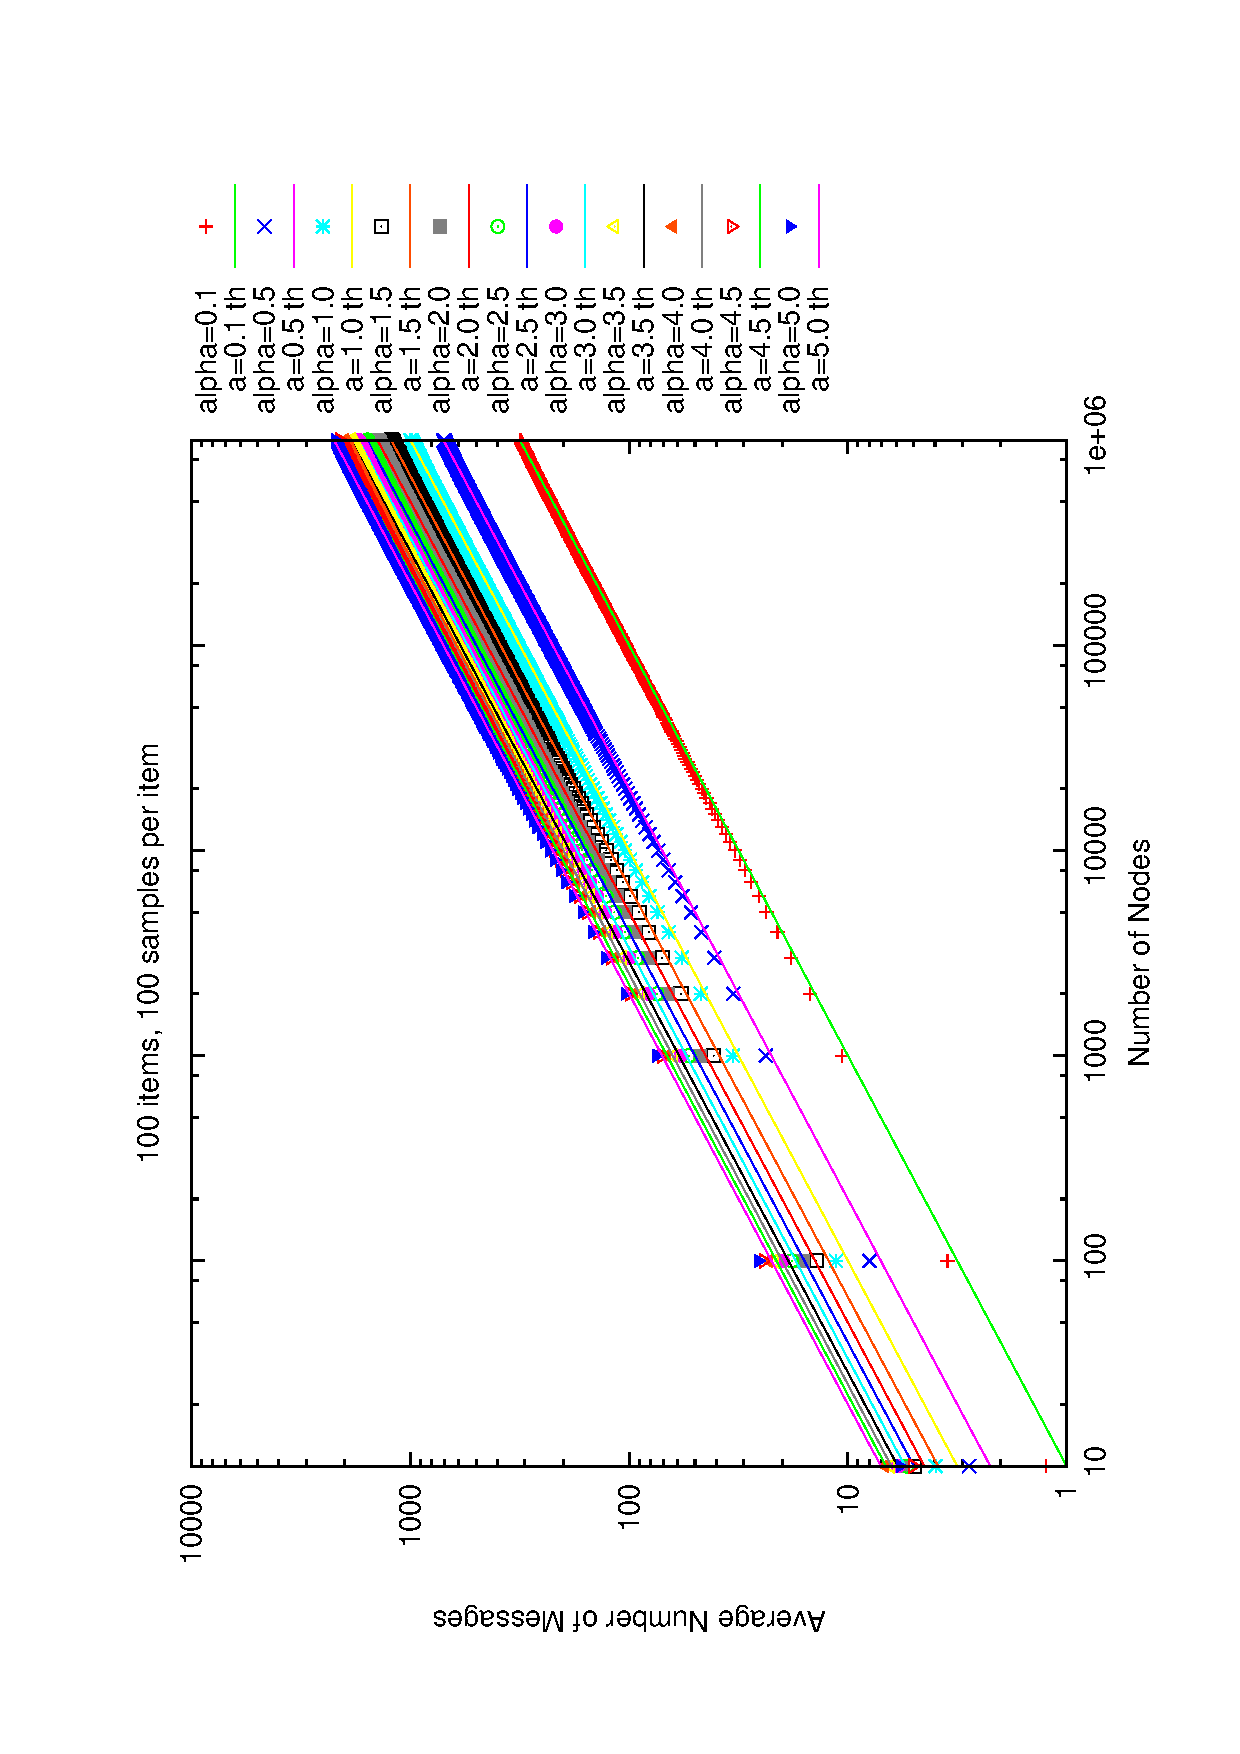
\includegraphics[angle=270,width=3.5in]{th_hops_loglog}
\caption{Query cost scales $O(\sqrt N)$. ''th" is for the theoretical result, 
and the other is the simulation result.} \label{fig:cost}
\end{figure}

%search time (depth)
For the search time, we measured the number of out-of-range links before finding 
a node in the range (by greedy routing) and the depth of the multicasting tree. Message 
transmission times at each link are assumed to be all the same. Figure \ref{fig:time} %\ref{fig:time5} 
compares simulation results with calculations with $\alpha$=1. 
As mentioned in Section \ref{sec:search_time}, 0.5 is substituted for $m$. 
Note that \textit{x} axis scales logarithmically. Our simulation shows a loose upper bound for search time, 
but it is obvious that the scaling of simulation result is more than 
$\log N$.
%solving  for m as optimal value, 1/2.....
\begin{figure}
\centering
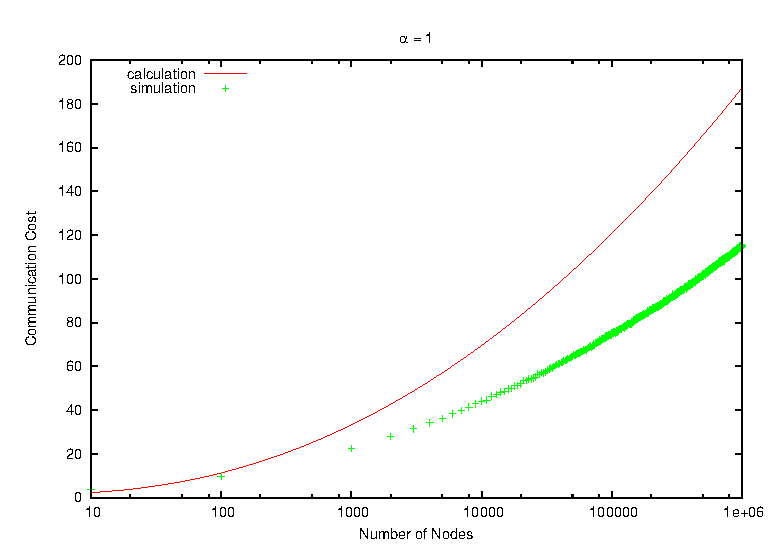
\includegraphics[width=3.5in]{time1}
\caption{Search time: We see our upper bound is loose, but the search time grows 
more than $\log N$, less than $\log^2 N$.} \label{fig:time}
\end{figure}

%\iffalse
%POB: Remove this for space concerns in the conference version,
%we'll put it back for the journal.

%\subsection{Communication Cost vs. Success Probability}
%\begin{figure}
%\centering
%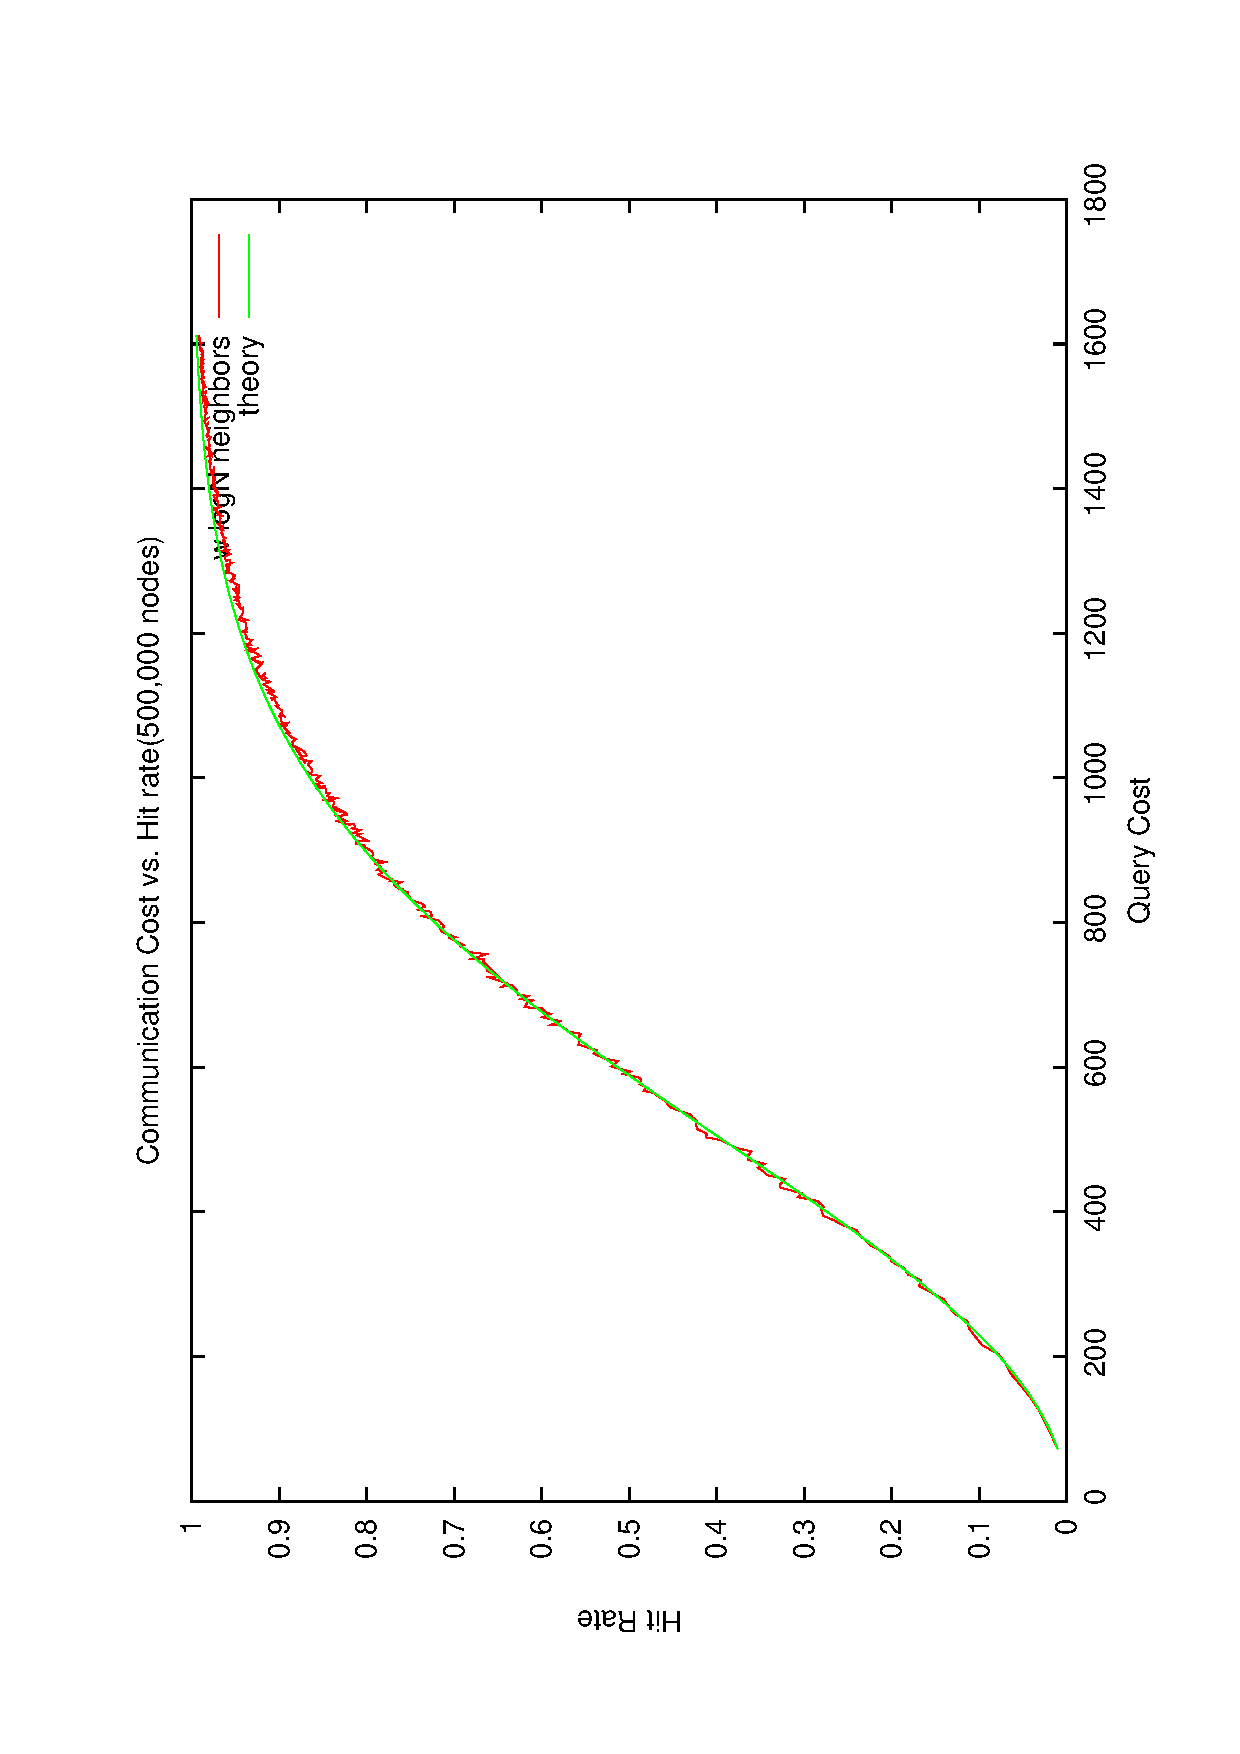
\includegraphics[angle=270,width=3.5in]{cost_hit_alpha_500k}
%\caption{} \label{fig:cost_hit}
%\end{figure}

\iffalse
\subsection{Numerical Analysis for Success Probability}
As described in Section \ref{sec:suc_prob}, the success probability remains constant 
regardless of the number of nodes in Deetoo network. However, 
the accuracy of network size estimation affects success probability.
The simulation results show slight trend downward of success probability as network size grows. 
The main reason for the slight decrease of success probability is that network 
growth makes variance of size estimation increase. In a bigger network, there are higher 
chances for a node to underestimate its network size relative to a small network. 
Underestimation is much more harmful for success probability because underestimation 
of the network size results in a narrower caching or querying range for bounded broadcasting. 
With the estimated network size distribution, 
we analyzed the impact of estimation on success probability numerically.  
We define $w_c$ and $w_q$ as the width of the the columns for caching and
querying respectively.  Since different nodes will initiate a cache and a
matching query, we can consider what happens when the two nodes have
difference estimates of the network size.

\begin{eqnarray*}
w_c \sqrt{B} = \sqrt{\alpha N} \\
w_c = \sqrt{\frac{\alpha N}{B}}
\end{eqnarray*}
Similarly, $w_q = \sqrt{\frac{\alpha N}{B}}$. 
Thus, the number of bins in overlap is:
\begin{eqnarray*}
w_c w_q = \alpha\frac{\sqrt{N_1 N_2}}{B}
\end{eqnarray*}
Assume that $N_1$ and $N_2$ are network size estimation for cache and query, 
respectively.
The success probability given a network size $N$ is:
\begin{eqnarray*}
P_{success}|N &=& \left(1-\frac{N}{B}\right)^{\alpha \frac{\sqrt{N_1 N_2}}{B}} \\
  &=& \left(1-\frac{N}{B}\right)^{\frac{N}{B}(\alpha \frac{\sqrt{N_1 N_2}}{N})} \\
  &\approx& 1-e^{\alpha \frac{\sqrt{N_1 N_2}}{N}}
\end{eqnarray*}
Finally, we calculate the success probability with given network size and
estimated distribution for both cache and query.  To do this, we need to know
the probability of estimating the size of the network given the actual size,
$P(N_1|N)$:
\begin{eqnarray*}
\langle P_{success} | N\rangle = \sum_{N_1=0}^{\infty}\sum_{N_2=0}^{\infty}P(N_1|N)P(N_2|N)\left(1-e^{\alpha \frac{\sqrt{N_1 N_2}}{N}}\right)
\end{eqnarray*}

\begin{figure}
\centering
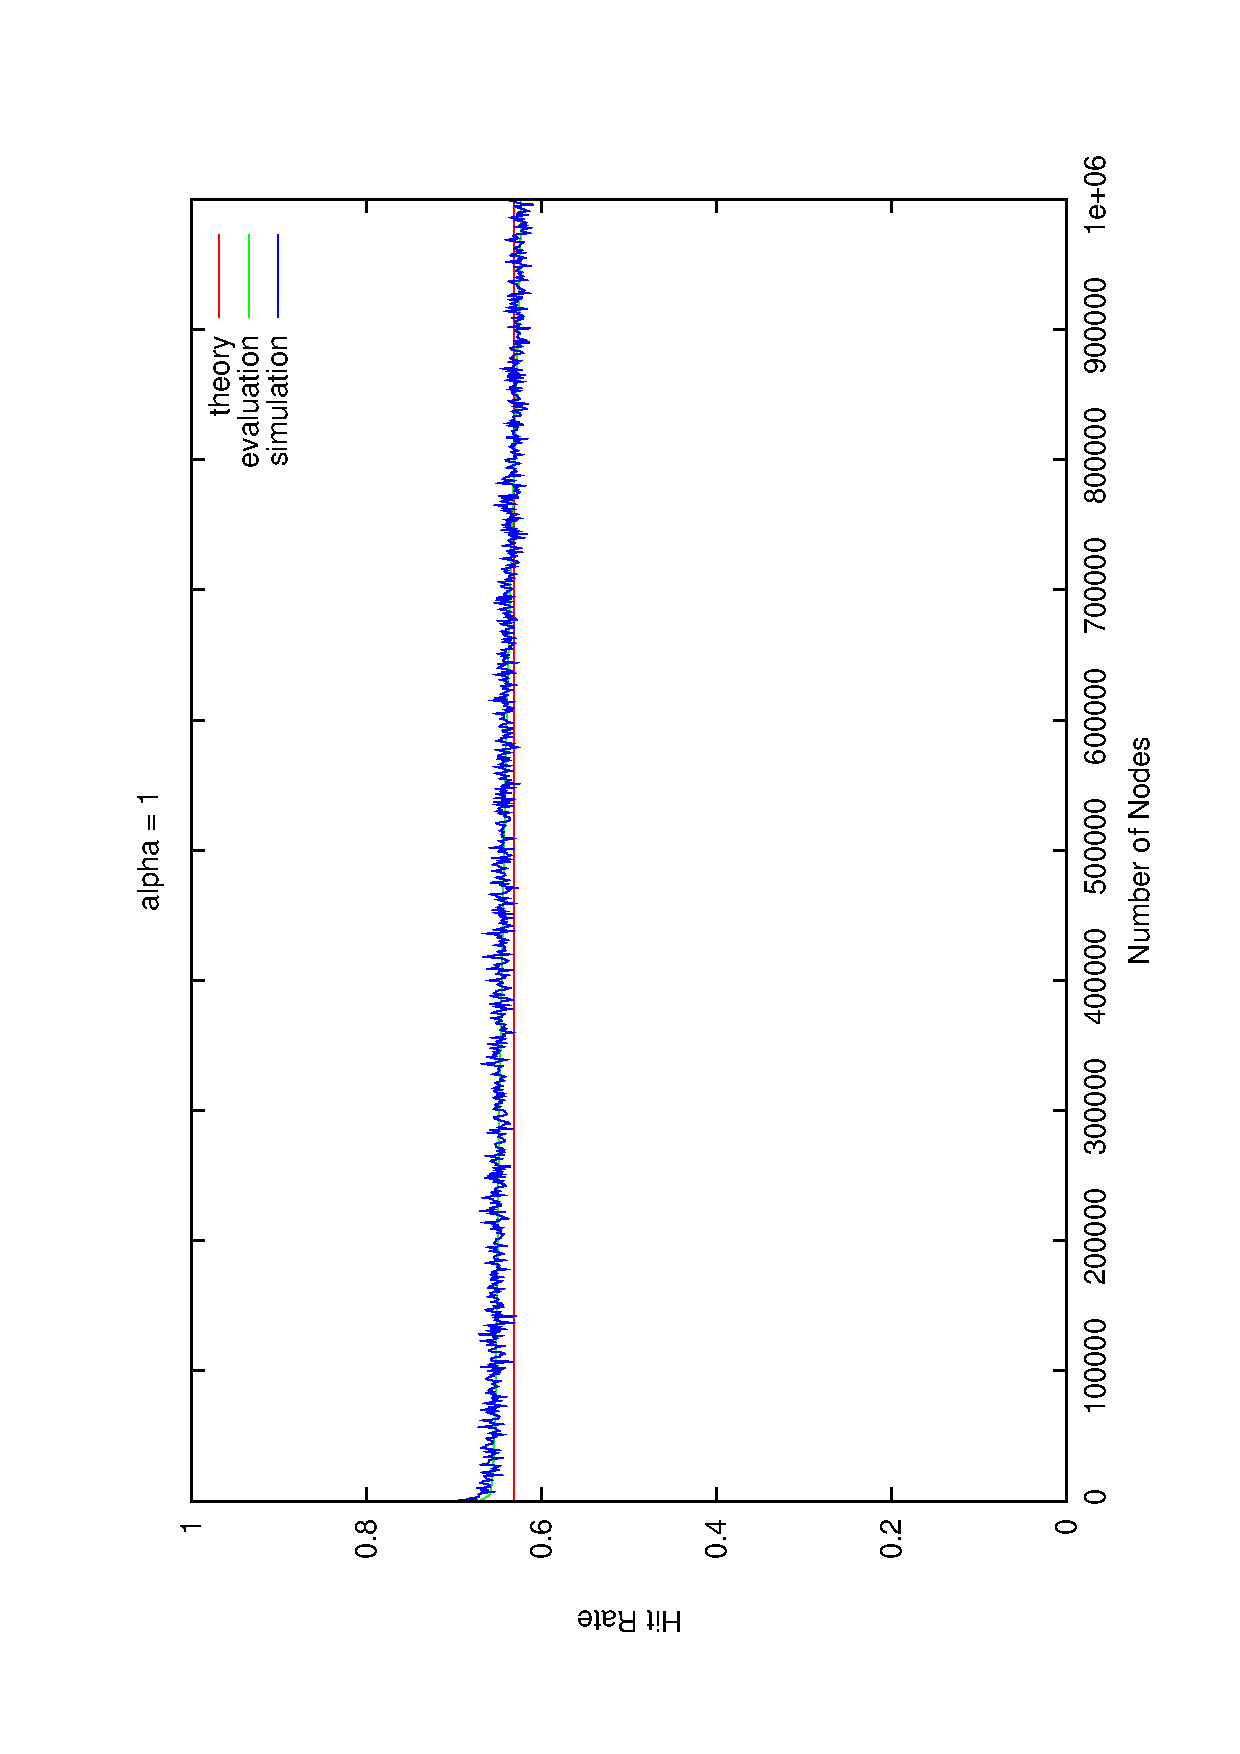
\includegraphics[angle=270,width=3.5in]{evaluation}
\caption{Success Rate decreases slightly as network size grows, 
while expected success rate stays constant. 
Estimation of the network size has bigger error margin in bigger 
networks. The simulation result depends on the estimation distribution.} 
\label{fig:anal}
\end{figure}
Using our simulation data to obtain $P(N_i|N)$,
figure \ref{fig:anal} shows that both the numerically evaluated success probability
and the simulation results for success probability decrease slightly 
as network size grows compared to the theoretical result, which assumes a global
knowledge of the network size. Even though there is some noise in the 
simulation results, we see that
the simulation result matches the numerical evaluation fairly well. Mean square error between numerical evaluation and 
simulation result is 3.93e-05.
\fi

\subsection{Robustness}
Due to the nature of P2P networks, each peer can leave or fail 
at any time. Therefore it is important to analyze the effect of node failures.
We will show that data objects are still accessible without generating 
excessive managing overheads under dynamic networks.
We extended Netmodeler%\cite{netmodeler} 
to model massive churn on nodes. 
The simulator setting is described below.
We set the network size first. Each node joins the network sequentially
following a uniform distribution.
Upon completing network formation with a given size, each node repeatedly 
leaves and joins.
%ambiguous
A node's rejoin time and leave time is exponentially distributed with same mean. 
%
The consequence of this distribution makes the average number of 
alive nodes in the system remains half of total number of the nodes 
originally joined. 
%As seen in the Figure \ref{fig:markov}, a 
A node's state transits 
between \emph{ON} and \emph{OFF} with probability of 0.5. In other words, 
the probability that each node is active at time t is $\frac{1}{2}$.
In our simulation setting, every node stays to be turned \emph{ON} until 
network size reaches a given number. 
%%confusing
It takes time a network size is saturated at the half of initial network size on average. 
%reason
%\begin{figure}
%\centering
%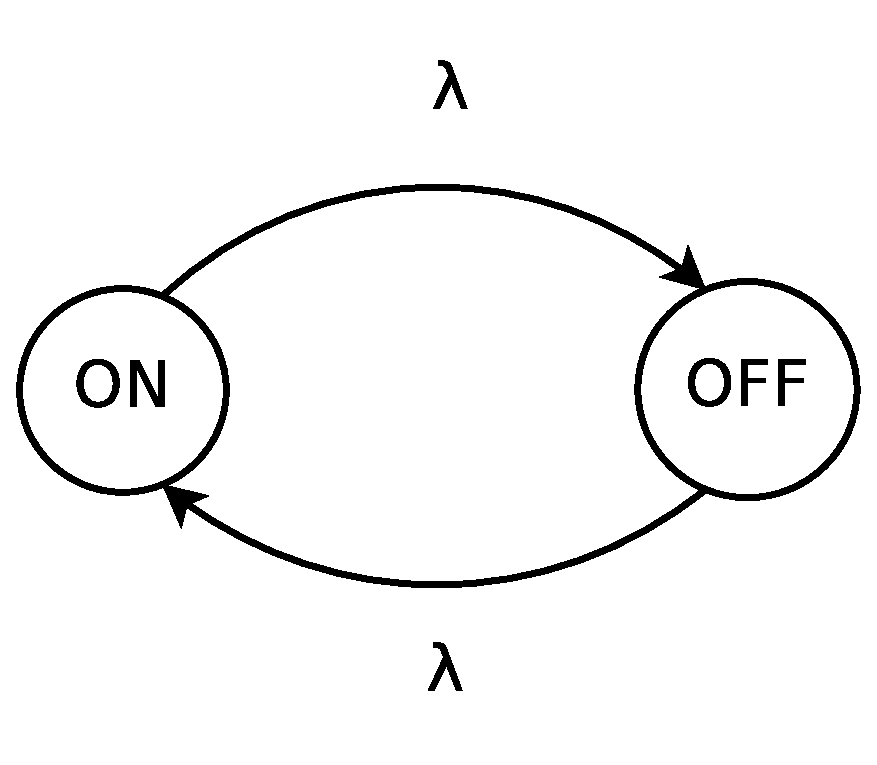
\includegraphics[width=2.5in]{queueingmodel}
%\caption{State Transition Diagram for each node. Because join time and leave time 
%distribution has same average, the probability that each node is alive 
%at a time t is 0.5.} \label{fig:markov}
%\end{figure}
After all nodes joined network, 100 data objects were inserted.
Queries were executed 100 times per data object. 
Both the cache events and the query events occur 
in a time distributed exponentially.
For simplicity, a replication factor, $\alpha$, is set to 1 
for the following simulations under churn.

\begin{figure}
\centering
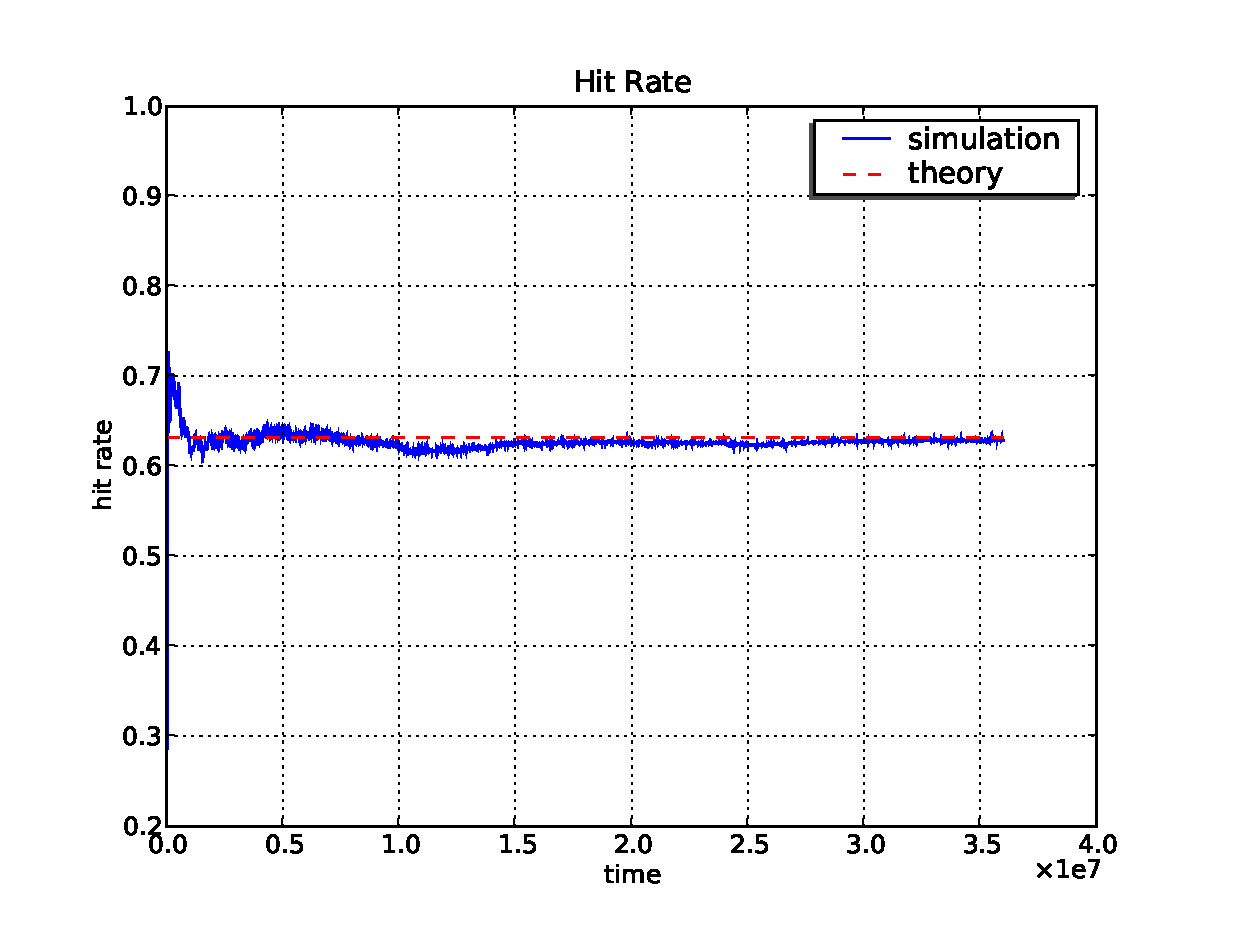
\includegraphics[width=3.5in]{hit_ch}
\caption{Success probability remains constant under Churn} \label{fig:hit_churn}
\end{figure}
Figure \ref{fig:hit_churn} demonstrates how the churn affects success probability.
Note that success probability remains constant. 
Also, the success probability still follows the theory as described in Section \ref{sec:suc_prob}.
This result shows that Deetoo is robust against network dynamics. 

\begin{figure}
\centering
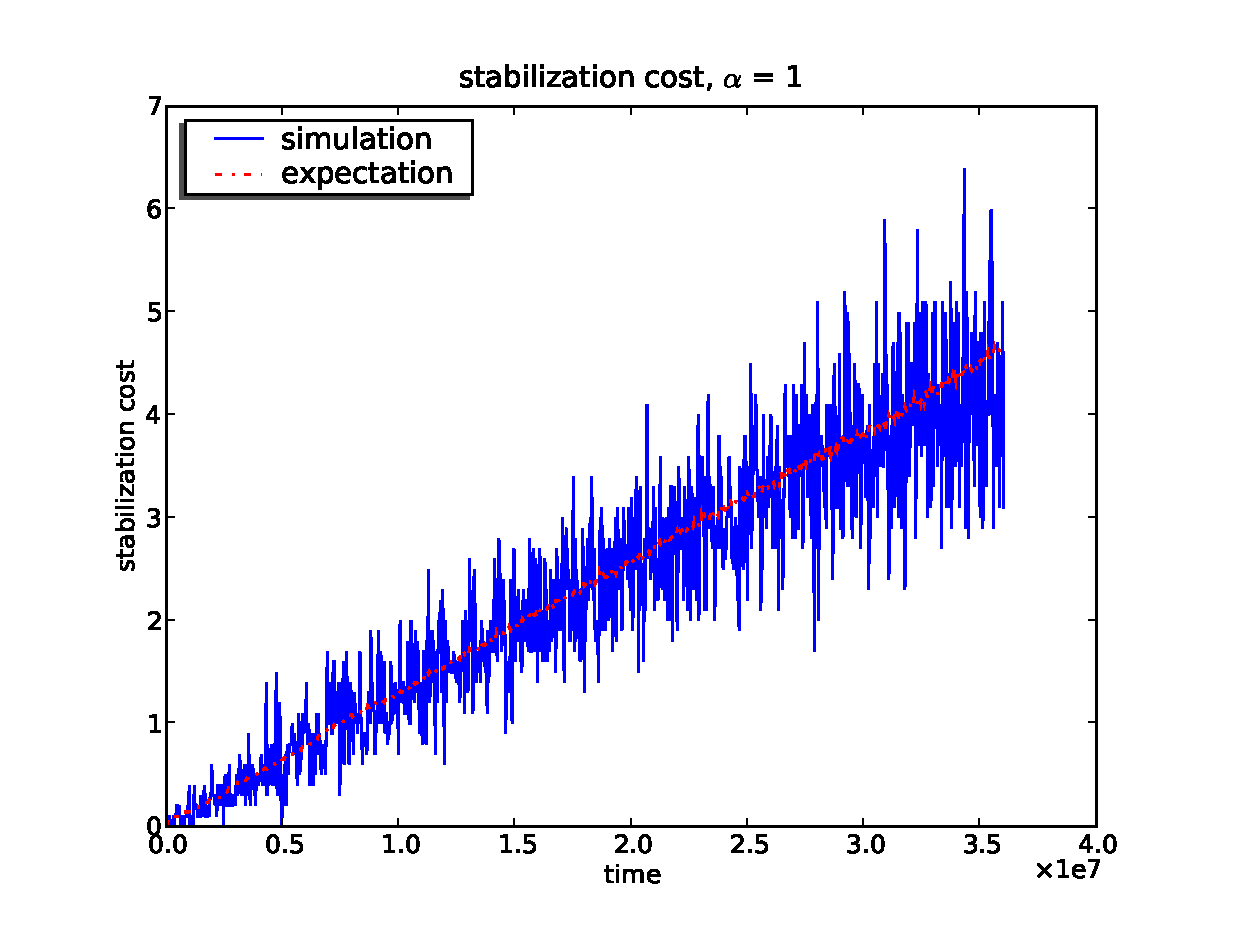
\includegraphics[width=3.5in]{stab_cost}
\caption{Stabilization Cost} \label{fig:stab_cost}
\end{figure}
Under the heavy churn in the network, message transfers for maintenance purposes
are not negligible. When a new node joins the network, it
is responsible for maintaining data objects if its address is within 
objects' range.
We counted what fraction of the total objects were transferred to a new node.
Assume that there are $k$ objects, and each are replicated over 
$\sqrt{N}$ nodes, we have $k$ $\sqrt{N}$ total objects in the system.
These objects are placed on nodes in the range selected uniformly at random, 
so the expected number of objects on each node is $k/\sqrt{N}$. 
Thus, joining cost is directly proportional to $1/\sqrt{N}$.

Figure \ref{fig:stab_cost} shows that how many replication occurred per unique
data object after joining new nodes. 
For the measure of stabilization cost, 
the size of network is set to 1,000 nodes initially. 
Note that stabilization cost grows not as time continues, but as the number of unique 
objects increases.
Unlike DHT-based stabilization, our process is much simpler, and costs less.
%explain more, what is DHT's cost? compare directly to our cost

With very low maintenance cost, Deetoo is capable of efficient data retrieval 
even under heavy churn.

\iffalse
\section{Applicable searches}
Structured P2P systems provide an efficient key-value look-up due to 
their hash table data structure.
Despite their efficiency, a DHT's data structure makes it challenging to answer new
types of queries.
When a new type of object or query is introduced, network topologies or 
caching strategies need to be redefined on structured systems. By comparison, 
unstructured systems can control new objects or queries without any modification. 
Unstructured systems make it possible to insert and retrieve 
different kinds of objects simultaneously over the same network.
The object type may be text, meta-data, image, audio, or video.
For example, Deetoo could be used for regular expression
matching, content-based search to find similar multimedia objects to
resolve some query object, or to perform SQL queries, XQuery or XPath searches of XML
documents. In the following subsection we describe the search process using 
regular expressions on top of Deetoo.
 
\subsection{Regular Expression Search}\label{sec:regex}
In this section, we present a practical search example which is one of many 
applicable searches with Deetoo.   
Regular expressions are used for searching strings of the text based on patterns. 
Objects might be strings, meta data of multimedia which are composed of strings, or 
objects' titles.
Managing data is not easy in decentralized and distributed 
networks which have no central control. In a distributed manner, there are critical issues 
to be overcome.
One issue is how to avoid transmission of multiple identical data 
from different peers to save bandwidth usage. 
Another issue is how to delete all the duplicated objects from the entire 
network when they are obsolete. 
Because objects are spread over the network due to Deetoo's caching property through  
bounded broadcasting, it is very important that all the replicated objects  
should be deleted when an original object needs to be deleted. 
It is assumed that each node maintains object records which include each object's ID, 
range information (start address, end address), and a replication factor ($\alpha$) as well as content.
The ID identifies data object and it is useful for deleting objects. 
The range information indicates the first address and the last 
of bounded broadcasting in a caching network. 
We explain how to apply operations for regular expression search on top of Deetoo.

\textbf{Object Insertion:} Objects or files are easily inserted into a network by 
bounded broadcasting as described in Section \ref{sec:broadcast}. $O(\sqrt{N})$ replicated objects 
reside in the network after insertion. 
Once an object is cached in the network, Deetoo requires to adjust the object's range information 
as the network size changes. Every time a new node joins the network, the node estimates network size. 
Before it copies an object from its neighbor, it calculates the object's range based on the 
estimated network size. With a replication factor ($\alpha$) in the object's record and the 
estimated network size ($N_{est}$), one can calculate a new range ($R=\sqrt{\alpha \frac{B}{N_{est}}}$).
The midpoint of the range ($M$) can be obtained by adding start and end addresses of the 
range from the object's record
and dividing by 2. Finally, $M+\frac{R}{2}$ and $M-\frac{R}{2}$ are the new start and end address 
of the range.
Then it compares it to the object's 
range information in the record. In accordance with a recalculated range, copied objects may be discarded 
from nodes or added to nodes.

\textbf{Search:}
When a node tries to find objects in corresponding to a given pattern, the node bounded-broadcasts 
the pattern in a randomly selected range. 
Users are able to select a searching method. There are three searching options, 
\textit{simultaneous, sequential}, and \textit{deleting}.
\begin{itemize}
\item \textit{Simultaneous} search uses bounded broadcasting. A pattern is transmitted 
to the nodes in the range. All matching results are transferred to a querying 
node simultaneously. This search method runs in time $O(log^2 N)$ and the querying node 
receives multiple replies.
\item \textit{Sequential} search is designed to avoid multiple answers from multiple peers.
A query sequentially visits a node in a tree under this option. 
First, a query starts bonded broadcasting to form a local tree. 
Figure \ref{fig:regextree} is an example of a local tree formed by bounded broadcasting. 
Children nodes having the matching object send results back immediately and the 
parent node waits for the first response from its children nodes. Upon receiving 
the first response, the parent node stops waiting for and transfers the result to a querying 
node. This process takes place recursively like depth-first search (DFS). 
The \textit{sequential} search option leads to an increase the searching time because nodes in the
tree are visited sequentially. The search time for sequential search is linear
in the range size, which is $O(\sqrt{N}$ in network size, while 
the simultaneous search takes at most $\log^2 N$ as described Section \ref{sec:search_time}.
At the expense of increased searching time, Deetoo prevents the generation of a large number of 
messages, and thereby it saves bandwidth utilization.
This option is especially useful for a popular object or a loosely defined regular expression search.
\item The \textit{deleting} option is used to delete objects from a network. 
The usage of this option is described in the following paragraph.
\end{itemize}

\textbf{Object Deletion:} Data deletion is more complicated than aforementioned operations.
This is because data are distributed over the network. In addition, peers cannot exactly identify 
how many replicated data exist in the network.
Thus, the Deetoo algorithm requires two stages of operations for deleting data objects from a network. 
First, Deetoo searches with the \textit{deleting} option 
in an arbitrary bounded broadcasting region in a querying ring. The \textit{deleting} 
option distinguishes a search for deletion from a plain search.
If there exists any node with a matching object, the node triggers the second stage, returning 
object's ID back to the asking node. 
In the second stage, the node starts bounded broadcasting the \textit{DELETE} command with the object's ID using 
the node's range information, and every node receiving the message discards the object whose ID matches.
Unlike the first stage, the second stage takes place in a caching ring because range 
information indicates the caching addresses.
We allow an asking node to use exact matching search rather than regular expression search. 
If regular expression search is utilized for the object deletion, 
certain similar objects that are not intended to be deleted can be eliminated. 
Consequently it would result in unexpected data loss.

\begin{figure}
\centering
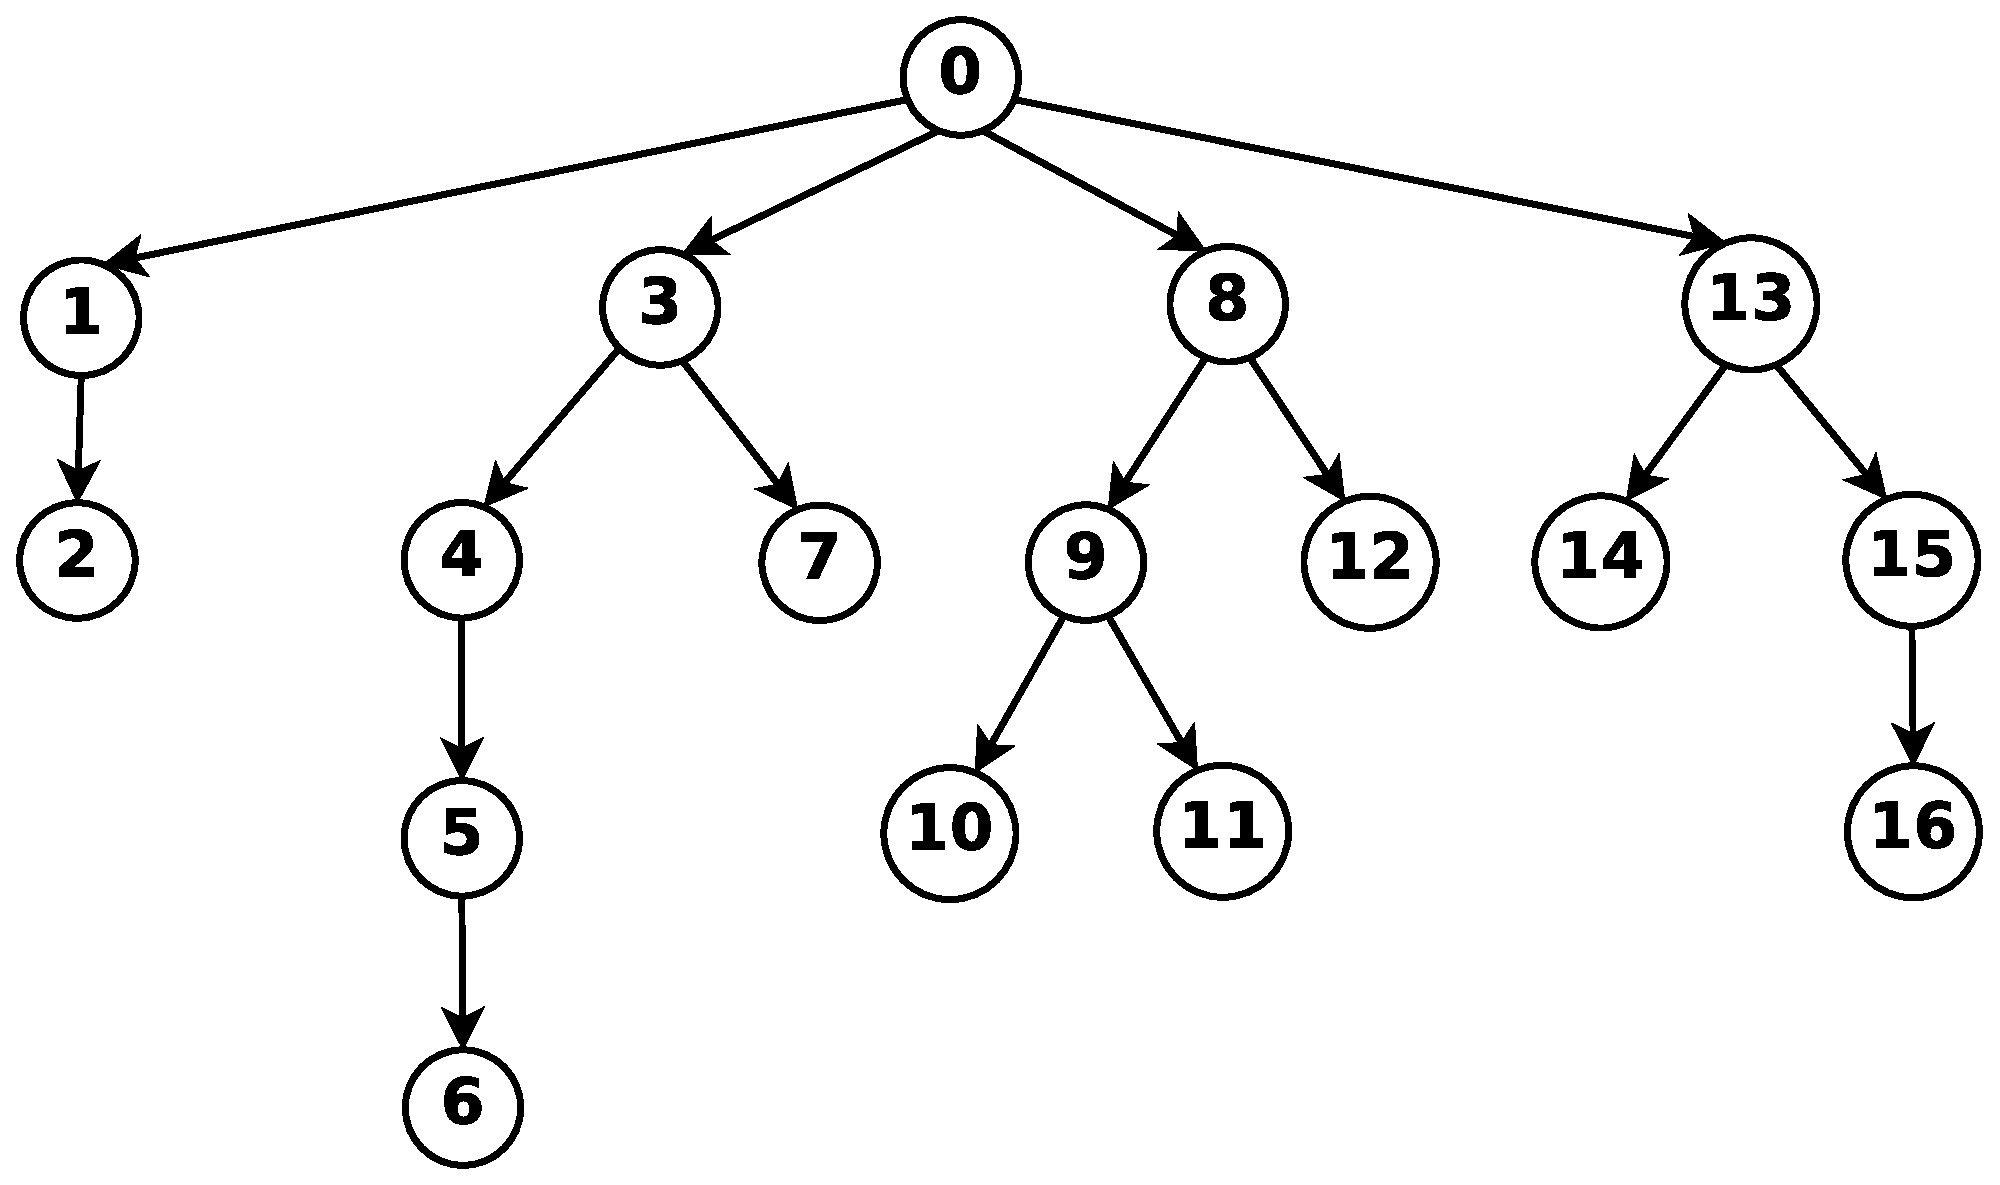
\includegraphics[width=3 in]{regextree}
\caption{Sequential Search: parent node only waits for the first response. For example, 
node 0 sends a query to node 1 instead of sending to all children node(node 1,3,8,13). 
If no response from node 1 is received, it sends a query to node 3. Node 0 obtains the first 
response, node 0 stops action and forwards the response to a querying node immediately.} 
\label{fig:regextree}
\end{figure}
\fi

\section{Conclusion and Future Work}
\label{sec:conclusion}
In this paper, we introduced Deetoo, a scalable routing peer-to-peer
protocol for unstructured networks which provides efficient caching
and lookup functionality with $O(1)$ query hit-rate, $O(\sqrt N)$
replication, $O(\sqrt{N})$ query cost, and $O(\log^2 N)$ search time.

Deetoo, allows objects to be updated and deleted, and can
be used to handle general queries.  Specifically, any problem
that can be mapped onto selecting (with high probability) objects
which match some query can be run over Deetoo.

In our future work, we plan to implement this routing algorithm
on Planet-Lab nodes and to investigate the performance under the presence
of frequently joining and leaving peers.  Additionally, due to the
fact that Deetoo is already a randomized algorithm, we are
investigating optimal approaches for dealing with lossy communications
such UDP/IP datagrams which go beyond naive hop-by-hop retransmission.

\bibliographystyle{IEEEtran}
\bibliography{d2}

\end{document}
